\chapter{Results of experiments with \sgp}
\label{app:sgp}
\textit{This Appendix presents graphically a summary of individuals runs using \sgp. Figures show a \textit{box-plot} representation for different strategies and a bar representation for the percentage of winner solvers types.}
\vfill
\newpage

In Figures~\ref{boxplot:5comm}, \ref{boxplot:8comm} and \ref{boxplot:9comm}, labels of the x-axis correspond to the following strategies:

\poslcaptiondesciption{
\begin{tabular}[t]{rl}
\textbf{NC}: & Non communication strategy\\
%\textbf{NC}: & Non communication strategy\\
\textbf{100SC1-1}: & 100\% of communicating solvers performing simple communication \oneTone \\
\textbf{50SC1-1}: & 50\% of communicating solvers performing simple communication \oneTone \\
\textbf{25SC1-1}: & 25\% of communicating solvers performing simple communication \oneTone \\
\textbf{100SC1-n}: & 100\% of communicating solvers performing simple communication \oneTn \\
\textbf{50SC1-n}: & 50\% of communicating solvers performing simple communication \oneTn \\
\textbf{25SC1-n}: & 25\% of communicating solvers performing simple communication \oneTn \\
\textbf{CC1-n}: & One set of solvers performing cyclic communication \oneTn \\
\textbf{CC1-n/2}: & Two sets of solvers performing cyclic communication \oneTn \\
\textbf{CC1-n/4}: & Four sets of solvers performing cyclic communication \oneTn \\
\textbf{100CC1-n}: & 100\% of communicating solvers performing cyclic communication \oneTone \\
\textbf{50CC1-n}: & 50\% of communicating solvers performing cyclic communication \oneTone \\
\textbf{25CC1-n}: & 25\% of communicating solvers performing cyclic communication \oneTone\\
\end{tabular}
}

Figures~\ref{barplot:5}, \ref{barplot:8} and \ref{barplot:9}, represent the percentage of winner solvers for each communication strategy, according to four different types:

\poslcaptiondesciption{
\begin{tabular}[t]{rl}
\receiver{Receiver}: & Receiver solver wining thanks to the received information \\
\sender{Sender}: & Sender solver \\
\nonreceiver{Pasive receiver}: & Receiver solver wining without using the received information \\
\textbf{Non communicating}: & Non communicating solver \\
\end{tabular}
}

%------ SELECTION
\begin{figure}[!h]
\centering
\subfloat[][\SGP{} 5-3-7 ]{
	\label{subfig:boxplot_sel5}
	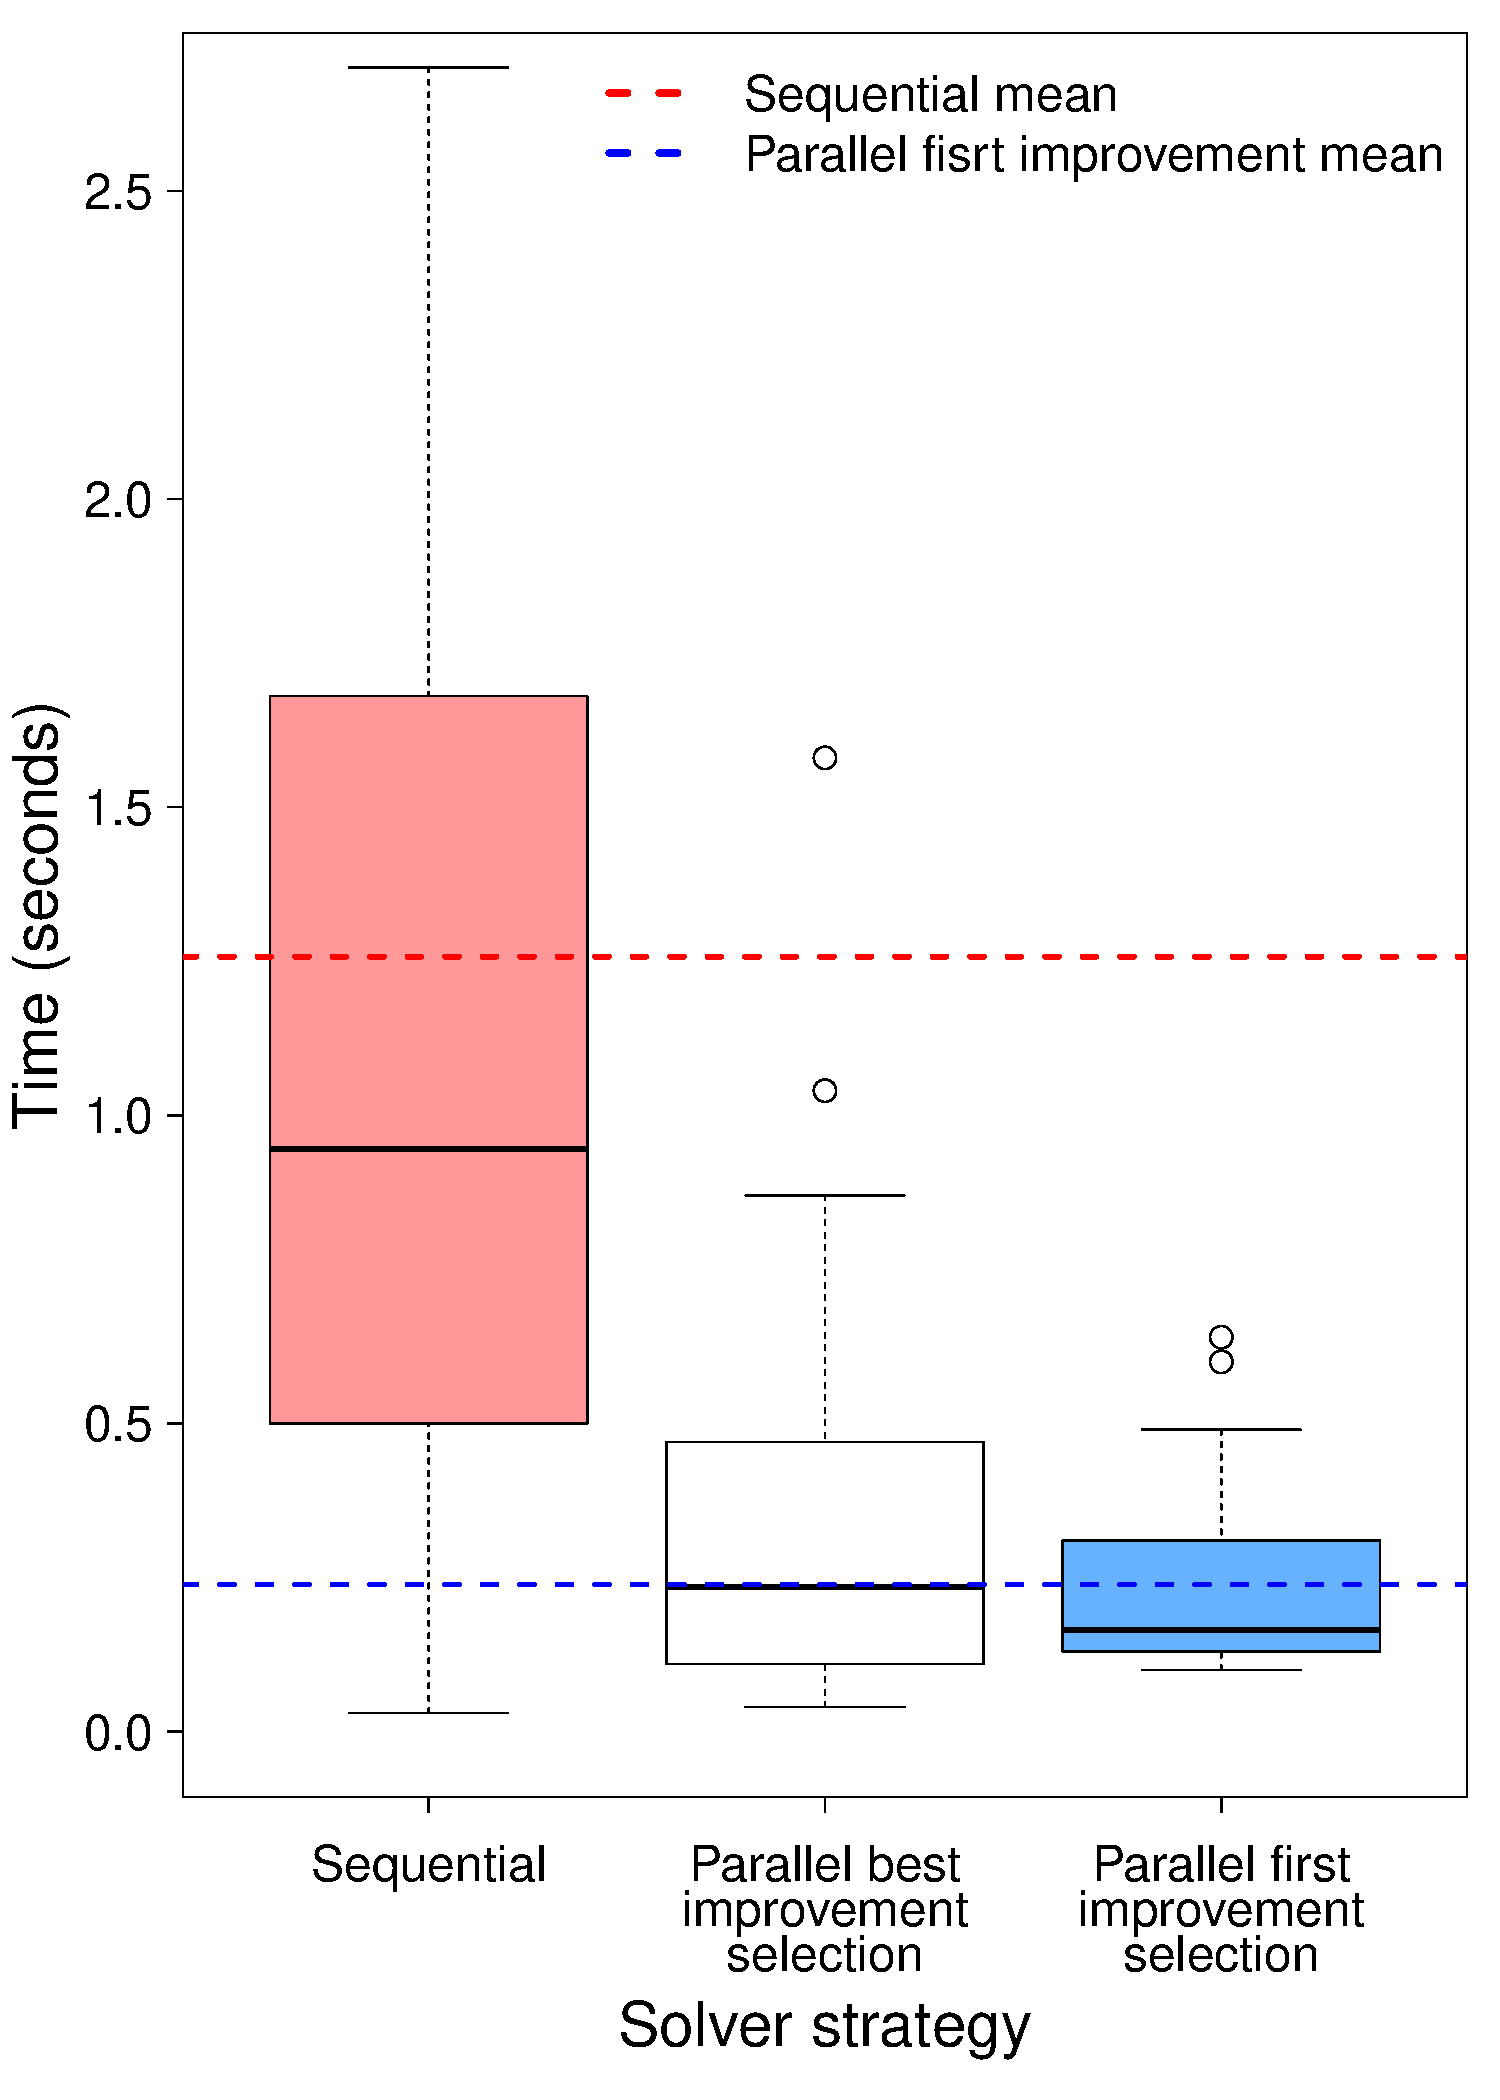
\includegraphics[width=0.4\linewidth]{g5_select_BP.pdf}
}\hspace{0.05\linewidth}
\subfloat[][\SGP{} 8-4-7 ]{%
	\label{subfig:boxplot_sel8}
	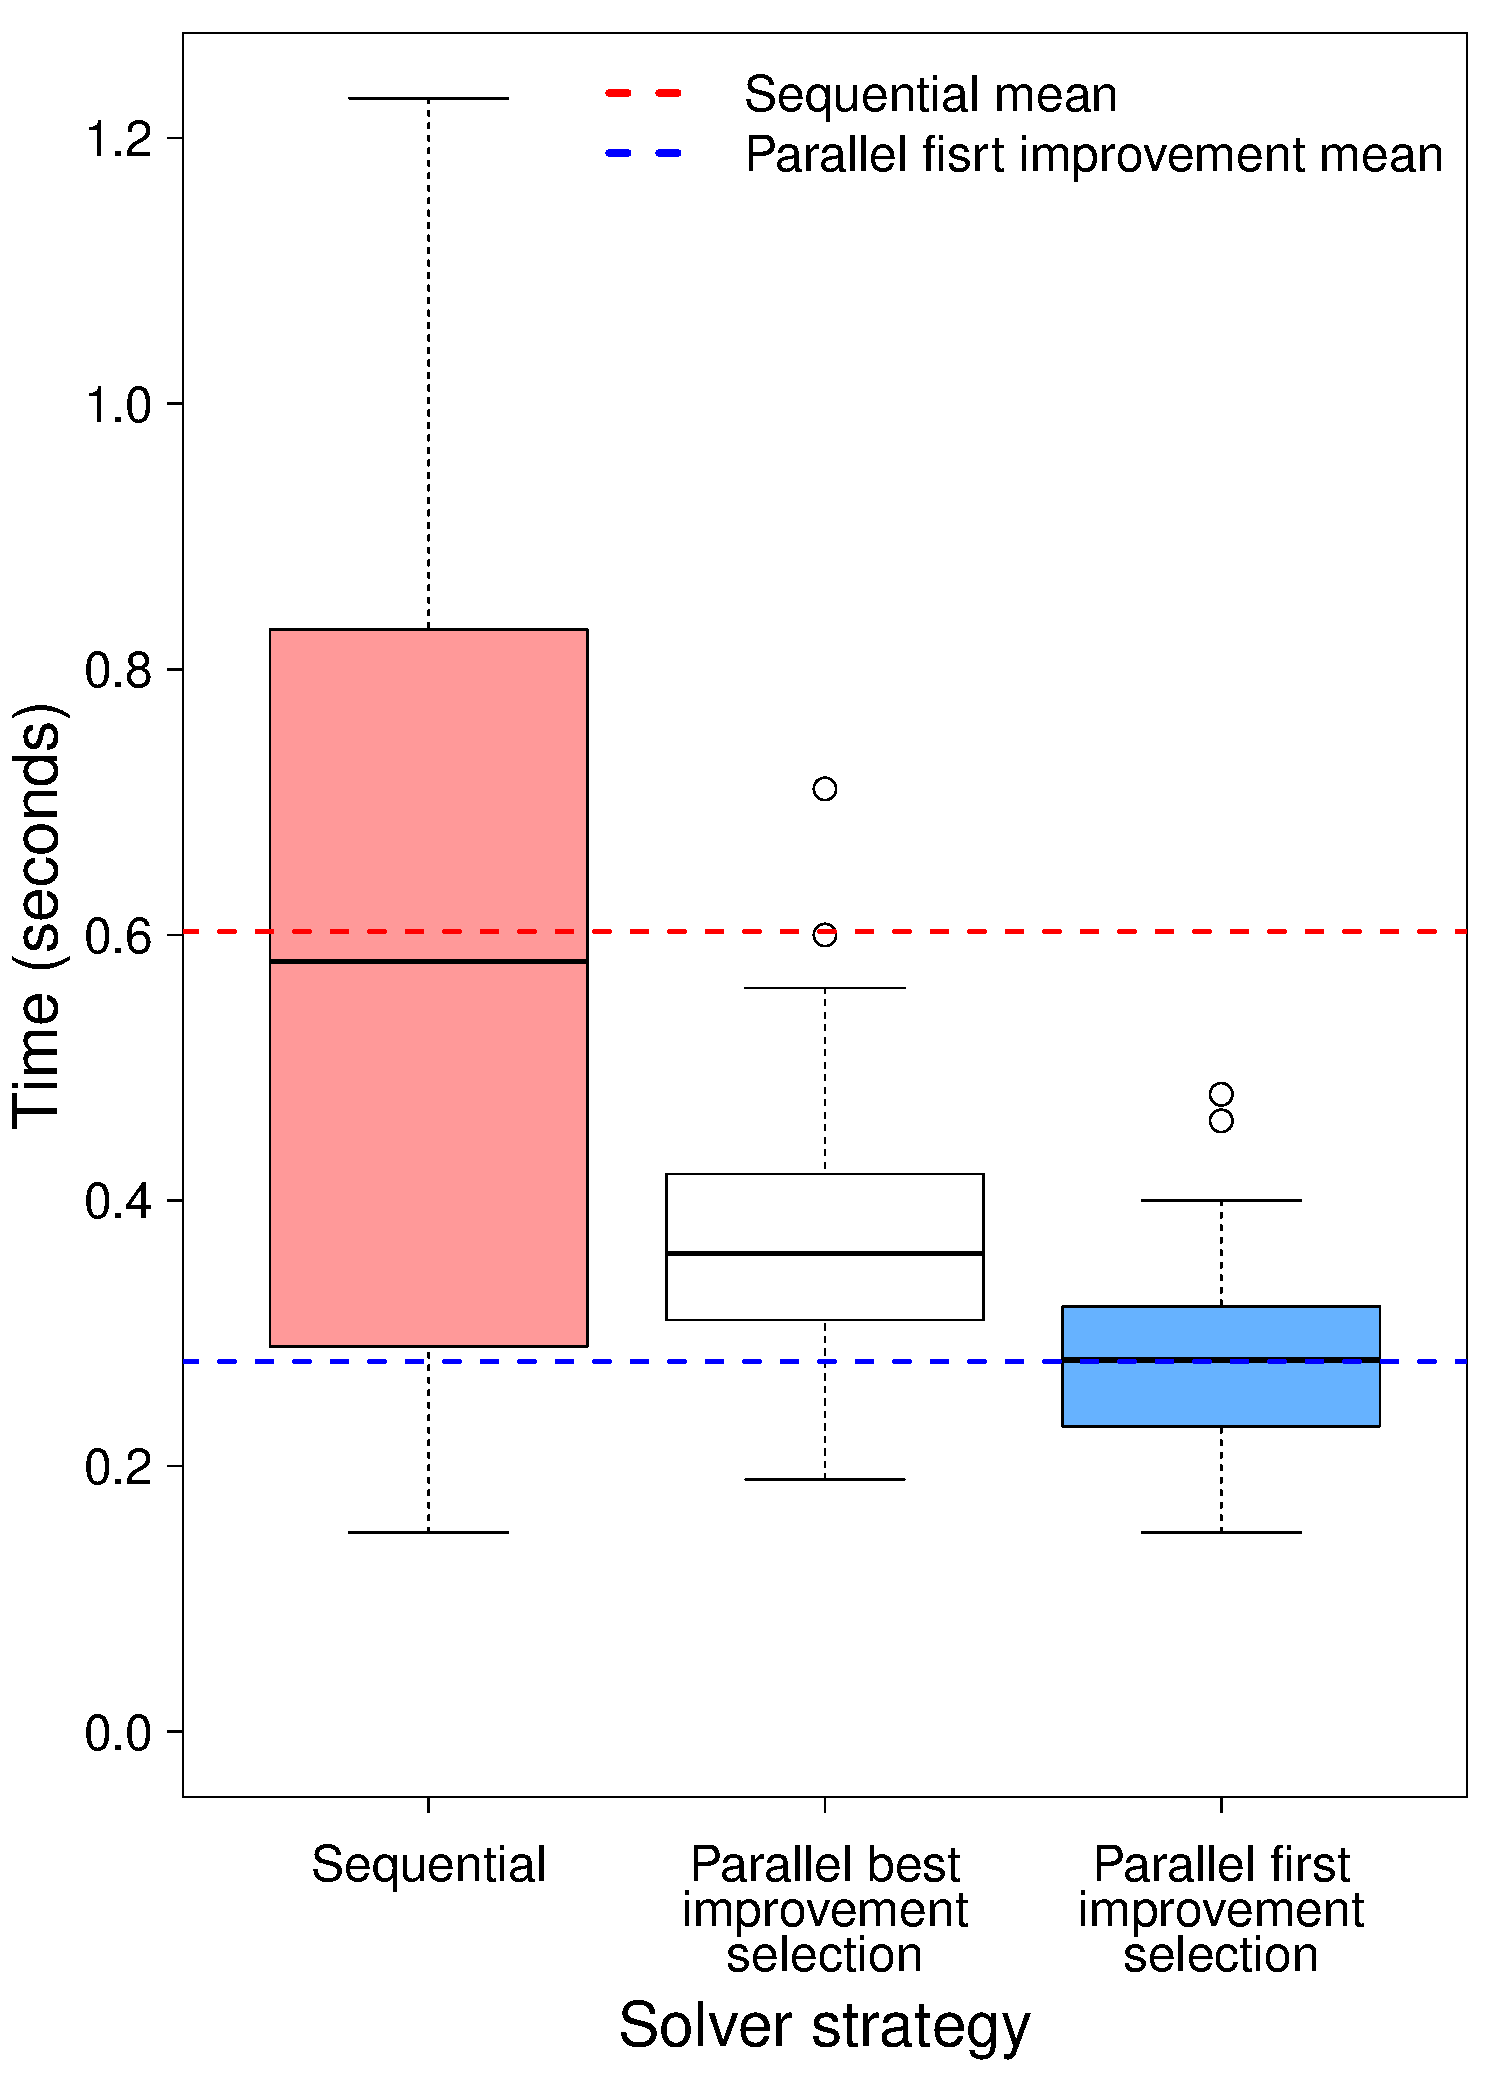
\includegraphics[width=0.4\linewidth]{g8_select_BP.pdf}
}\\
\subfloat[][\SGP{} 9-4-8 ]{%
	\label{subfig:boxplot_sel9}
	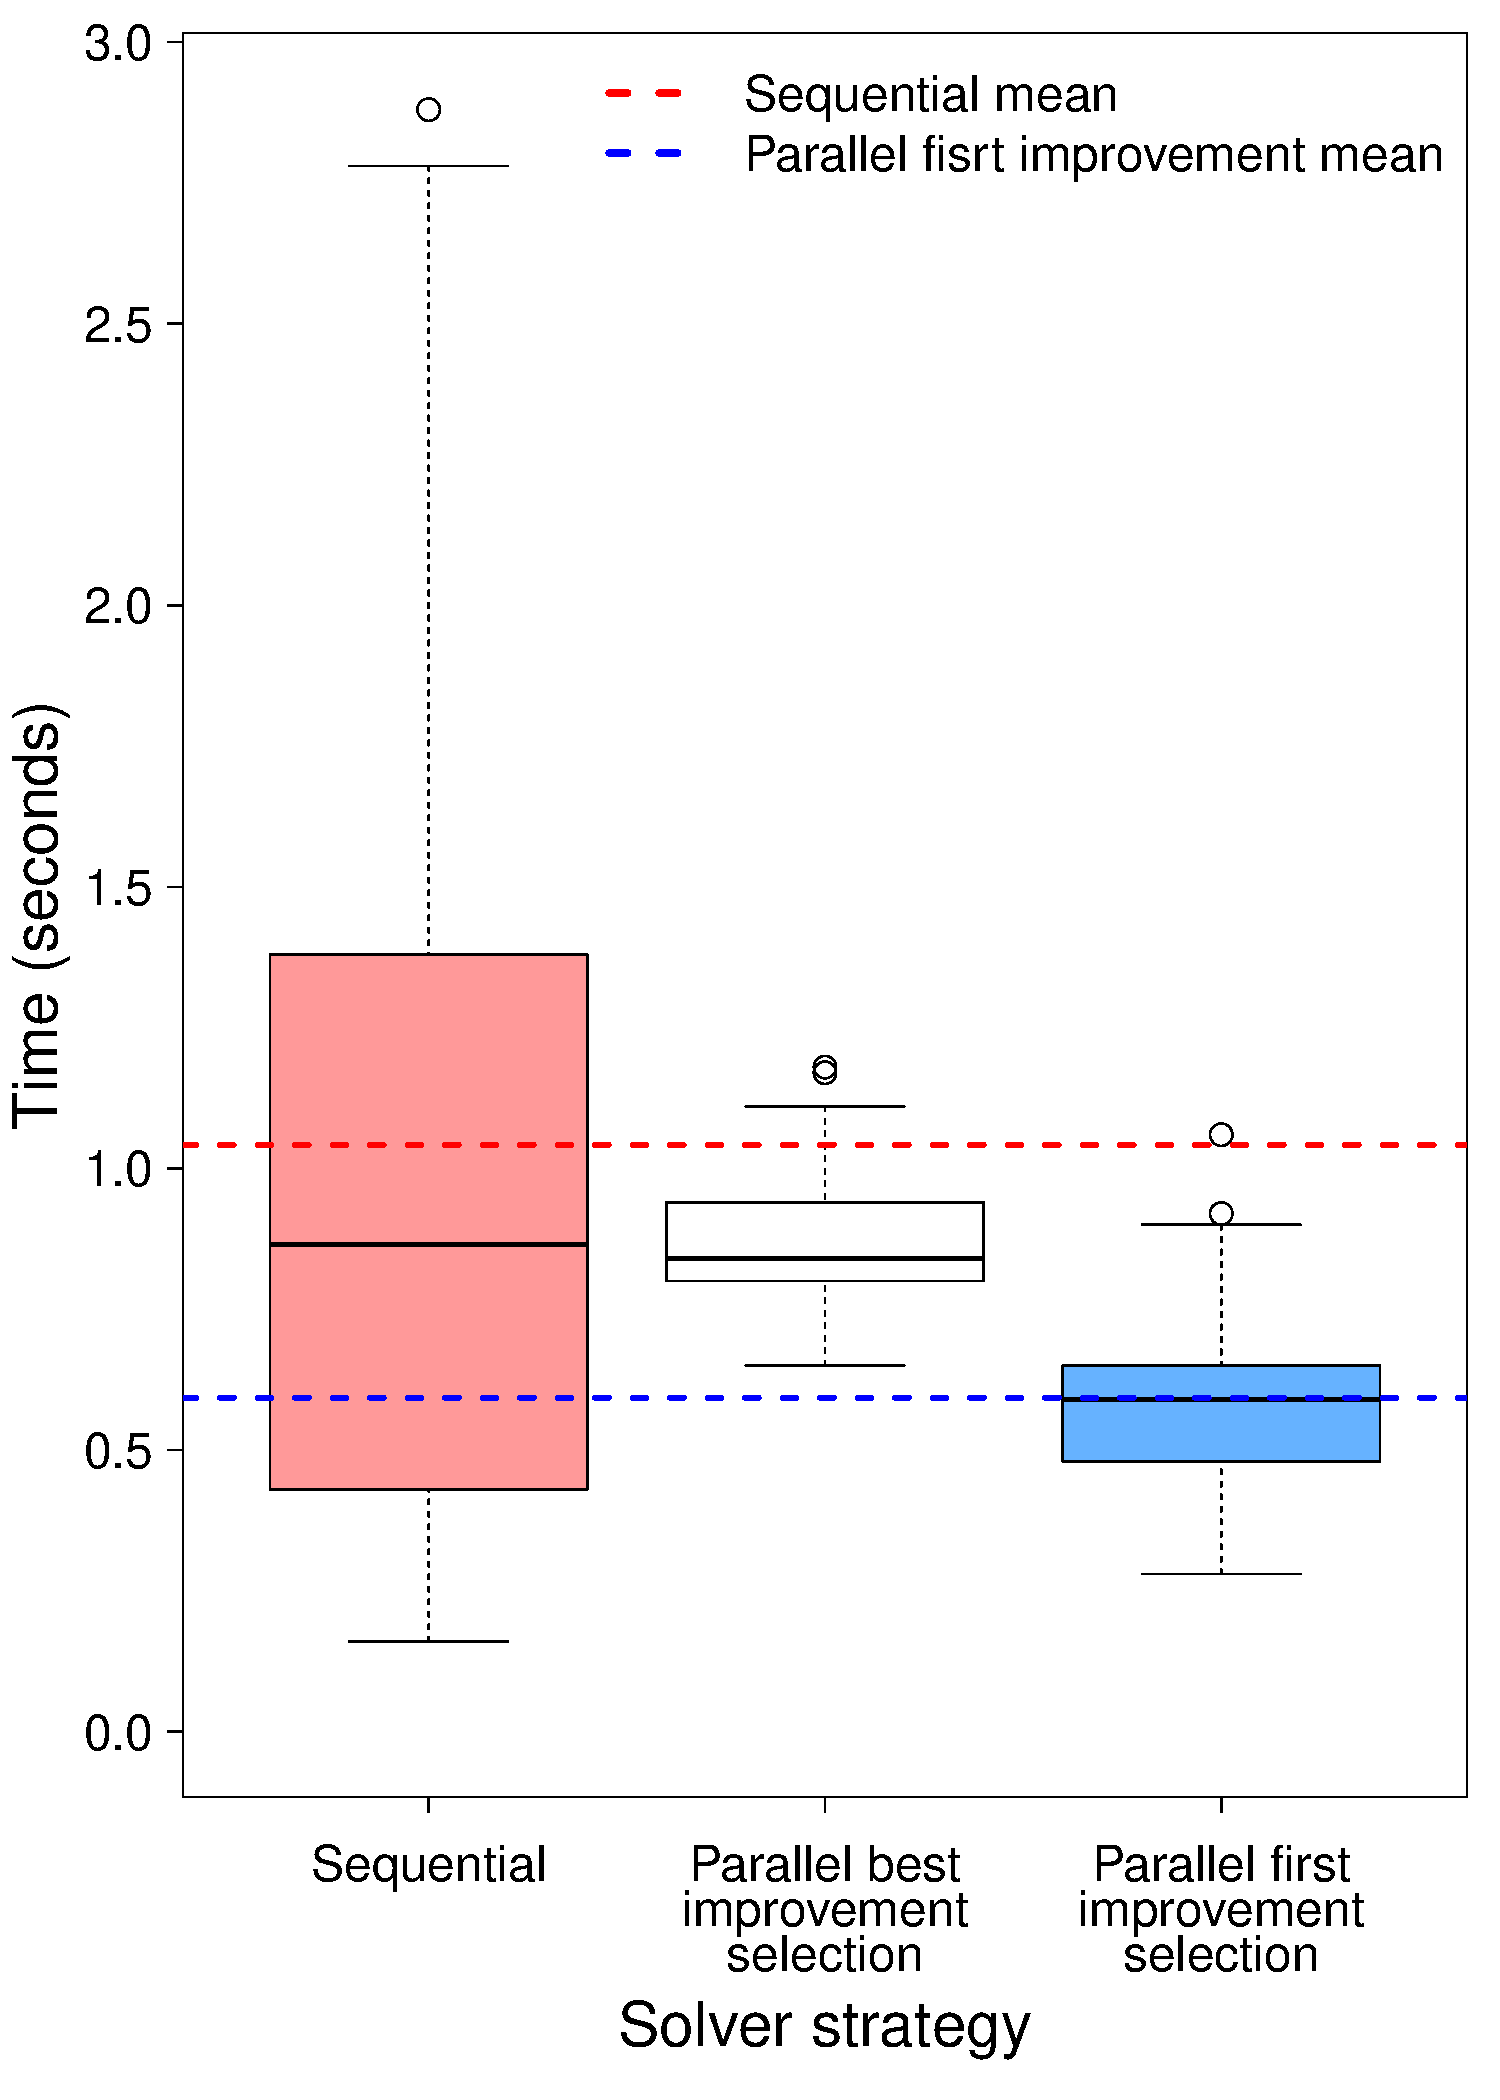
\includegraphics[width=0.4\linewidth]{g9_select_BP.pdf}
}
\caption[]{Comparison between sequential and parallel (best improvement and first improvement selections) runs to solve \SGP{} using \posl}
\label{fig:boxplot_sel}
\end{figure}

%------ COMMUNICATION
\begin{figure}[!h]
\centering
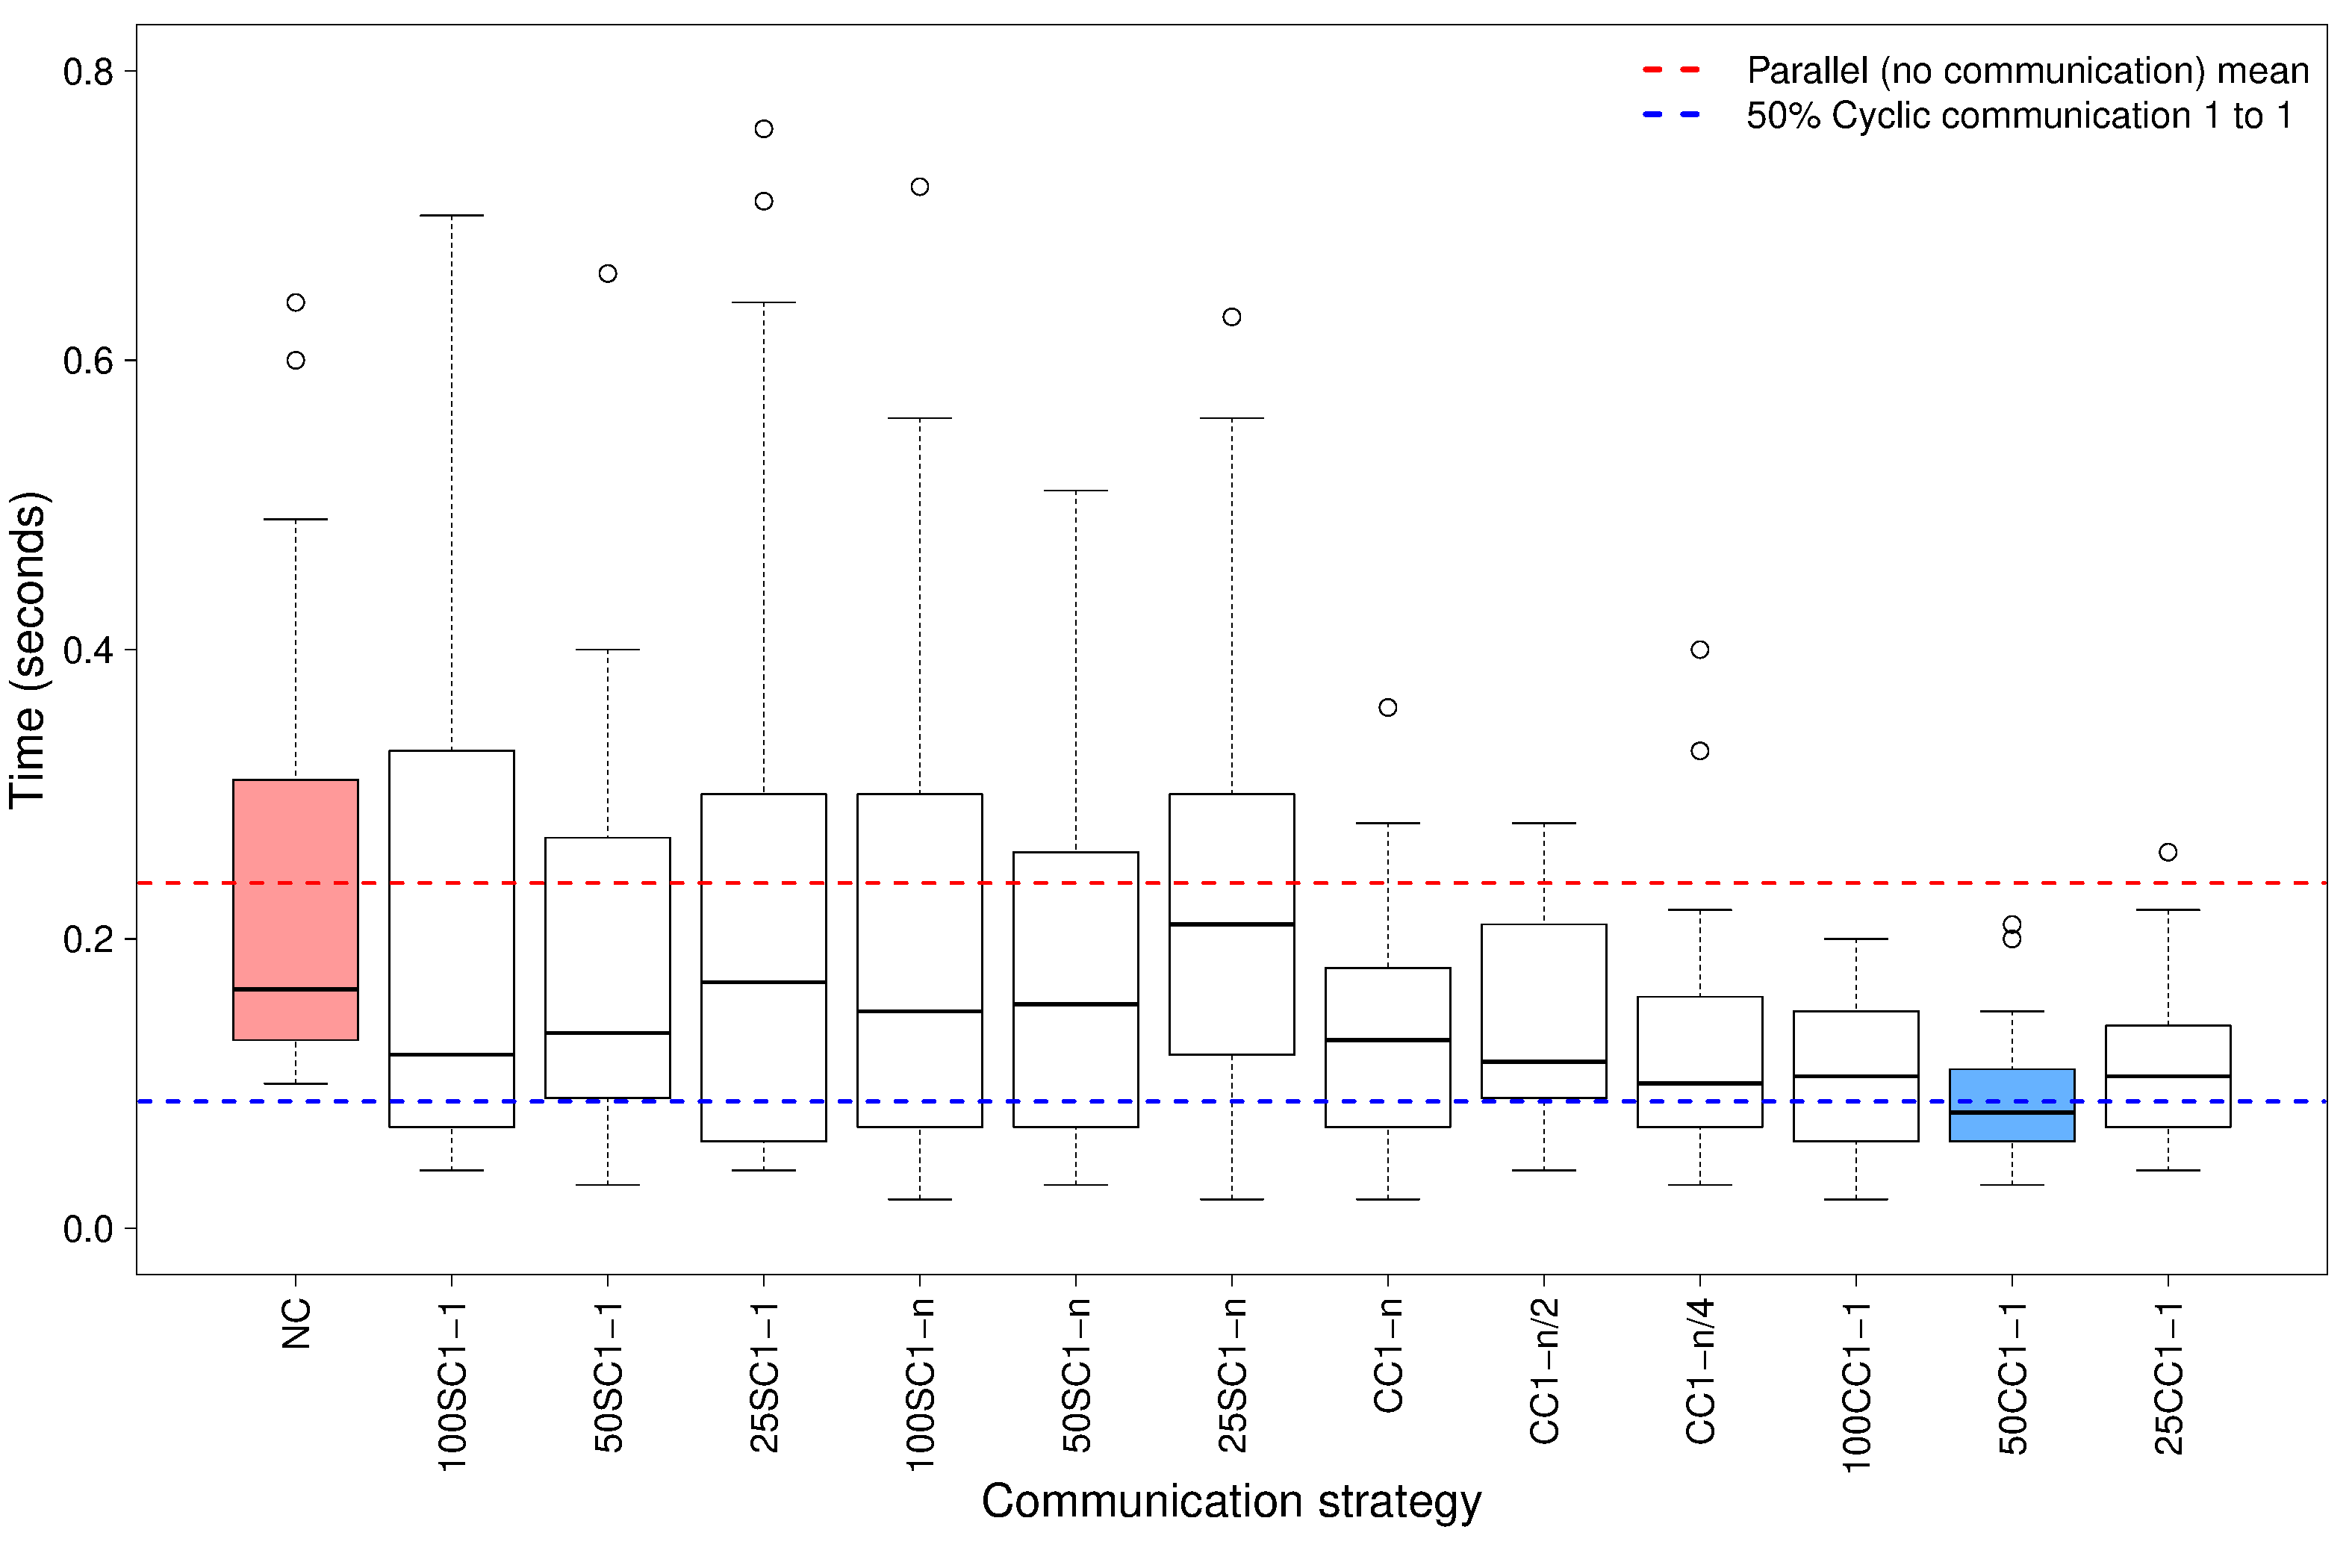
\includegraphics[width=0.8\textwidth]{g5_comm_BP.pdf}
\caption{Different communication strategies to solve \SGP{} 5-3-7 using \posl}\label{boxplot:5comm}
\end{figure}

\begin{figure}[!h]
\centering
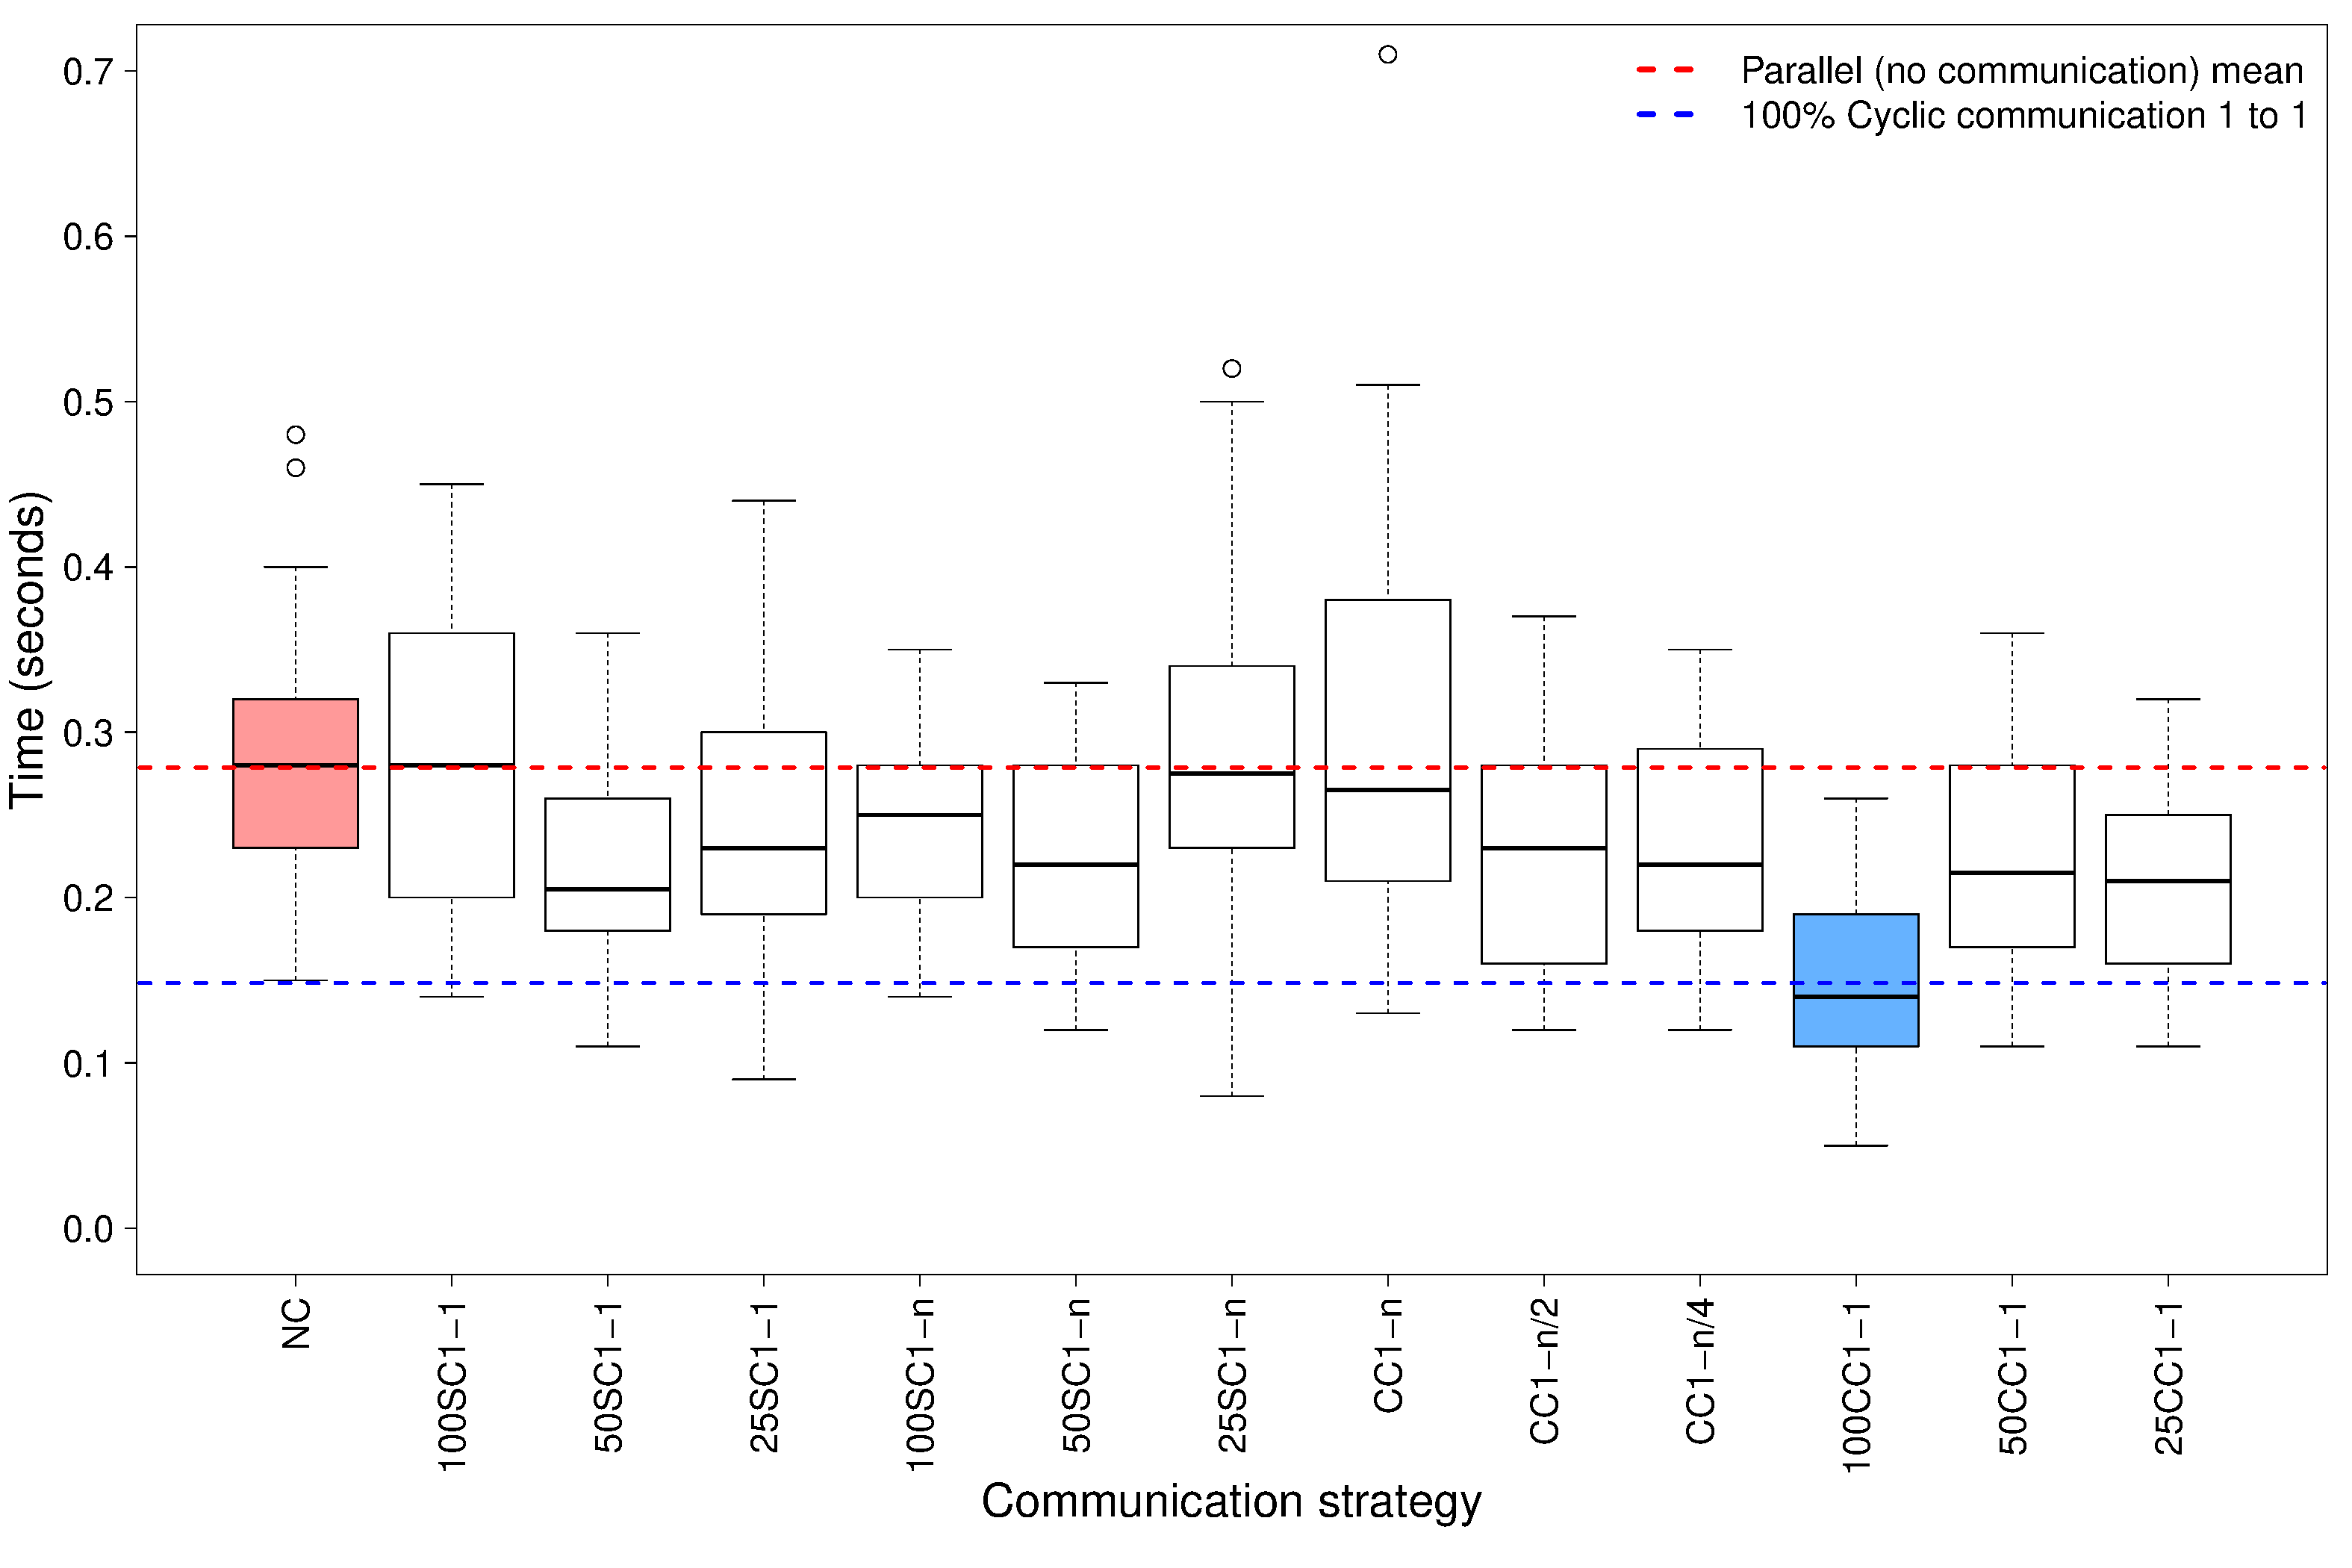
\includegraphics[width=0.75\textwidth]{g8_comm_BP.pdf}
\caption{Different communication strategies to solve \SGP{} 8-4-7 using \posl}\label{boxplot:8comm}
\end{figure}

\begin{figure}[!h]
\centering
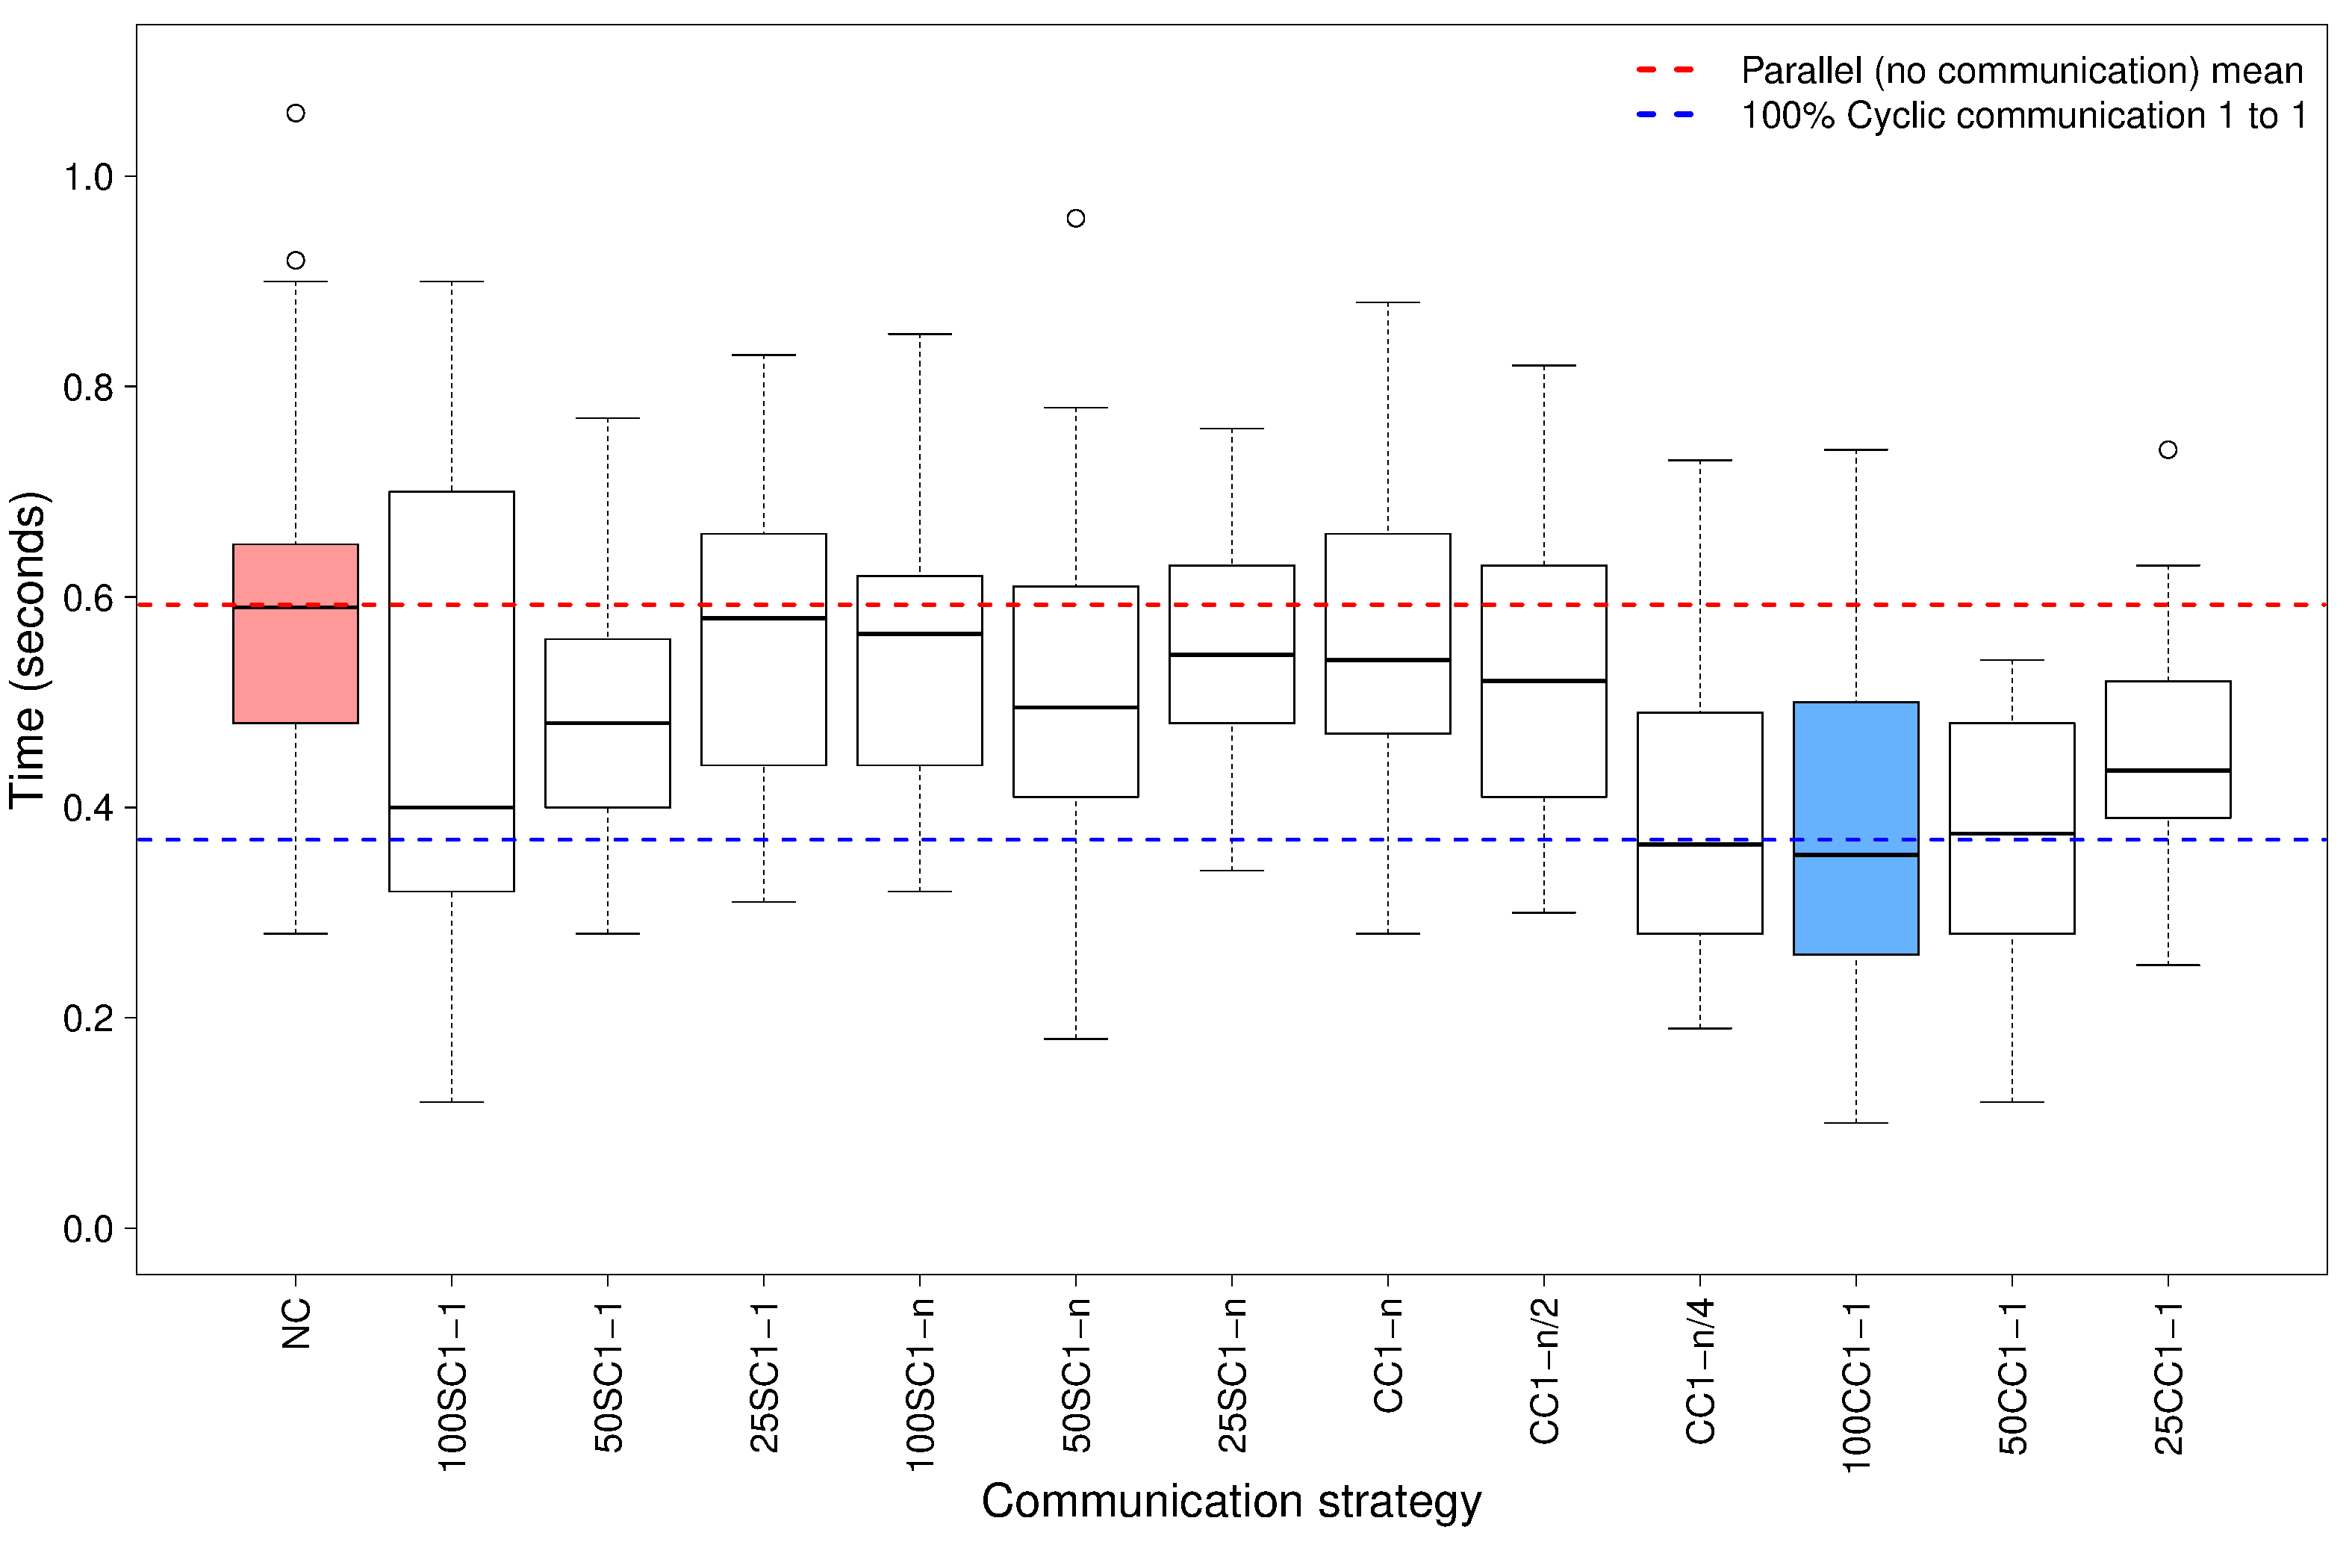
\includegraphics[width=0.75\textwidth]{g9_comm_BP.pdf}
\caption{Different communication strategies to solve \SGP{} 9-4-8 using \posl}\label{boxplot:9comm}
\end{figure}

%\begin{figure}[!h]
%\centering
%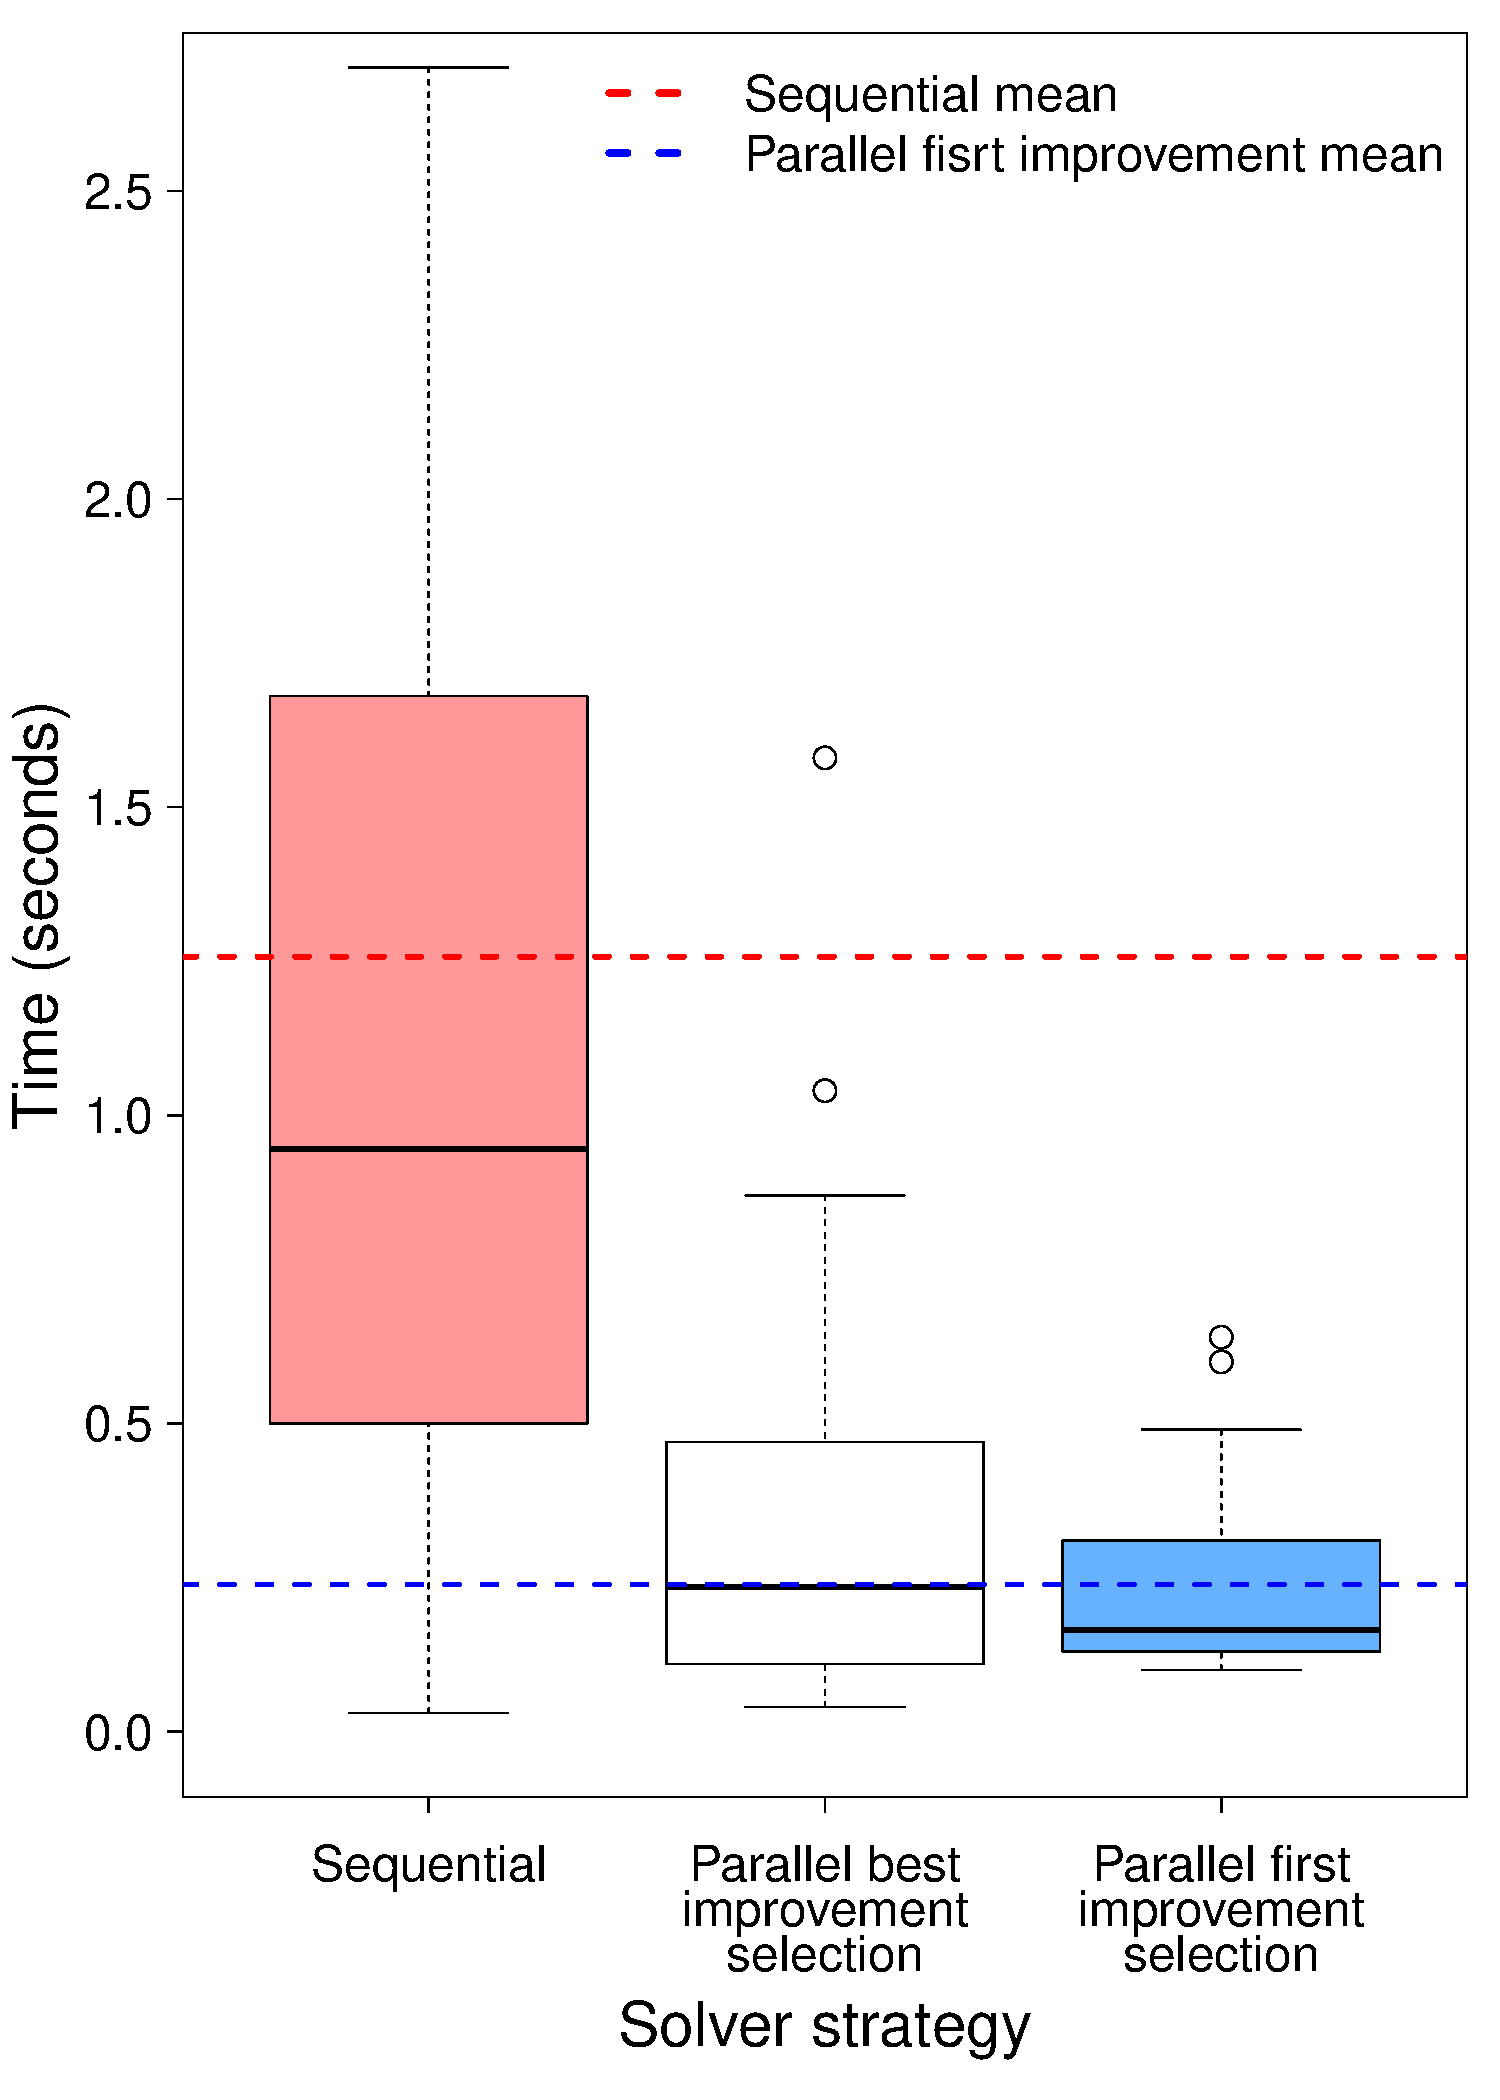
\includegraphics[width=0.4\textwidth]{g5_select_BP.pdf}
%\caption{Comparison between sequential and parallel (best improvement and first improvement selections) runs to solve \SGP{} 5-3-7 using \posl}
%\end{figure}

%\begin{figure}[!h]
%\centering
%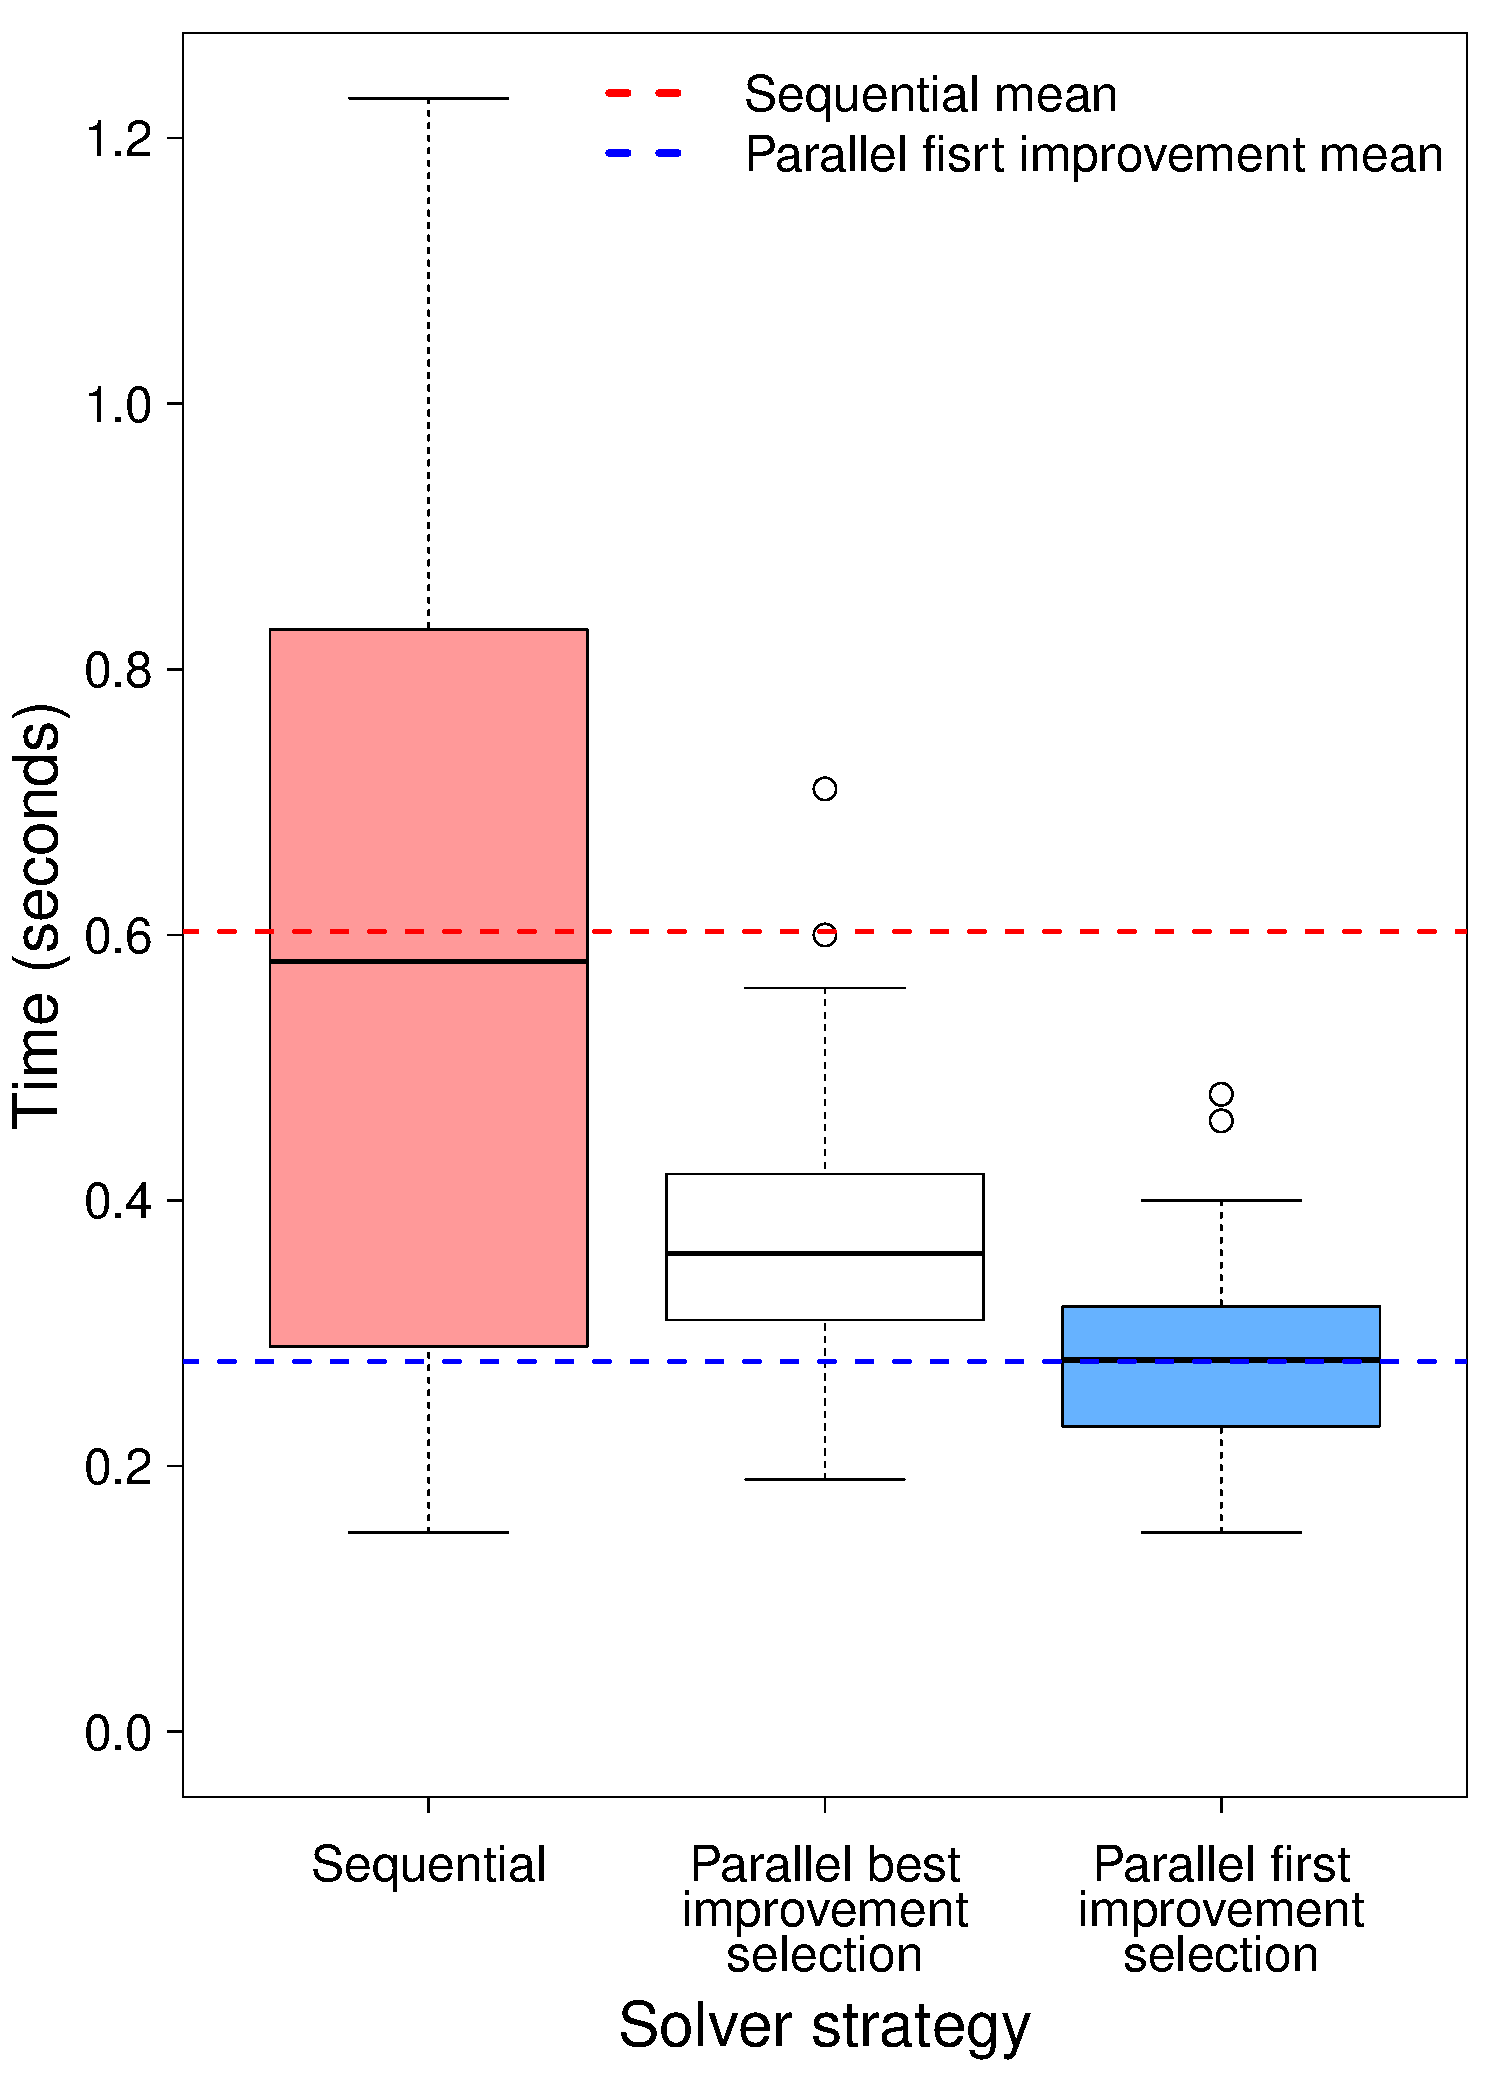
\includegraphics[width=0.75\textwidth]{g8_select_BP.pdf}
%\caption{Comparison between sequential and parallel (best improvement and first improvement selections) runs to solve \SGP{} 8-4-7 using \posl}
%\end{figure}

%\begin{figure}[!h]
%\centering
%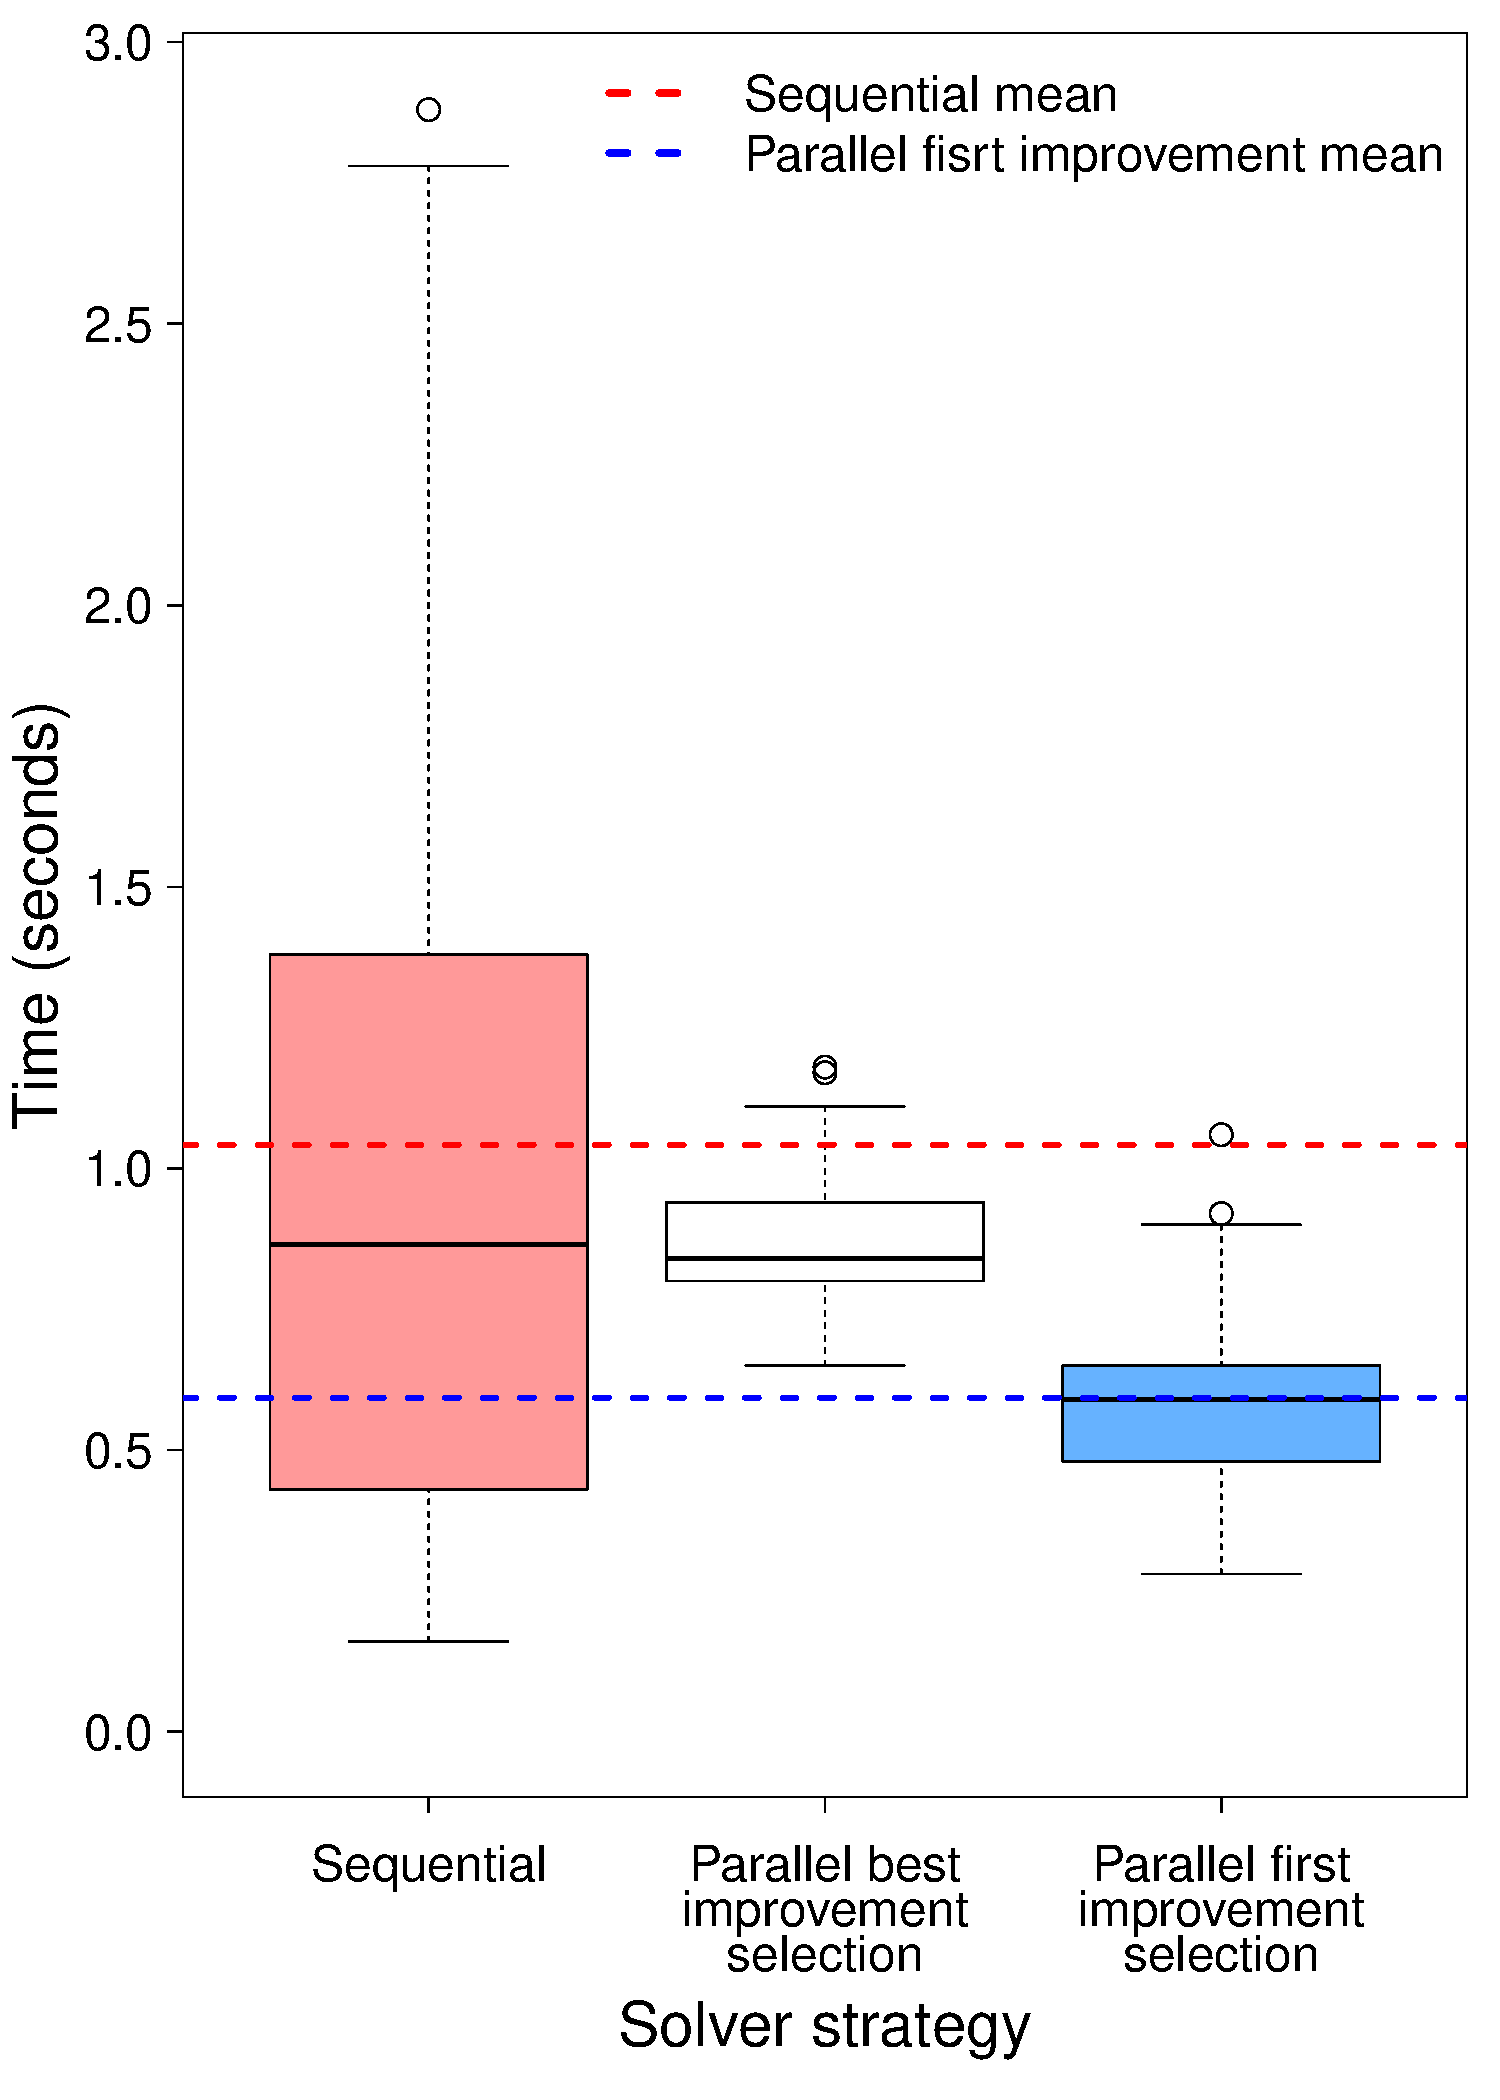
\includegraphics[width=0.75\textwidth]{g9_select_BP.pdf}
%\caption{Comparison between sequential and parallel (best improvement and first improvement selections) runs to solve \SGP{} 9-4-8 using \posl}
%\end{figure}


%-------- SOLVER TYPE
\begin{figure}[!h]
\centering
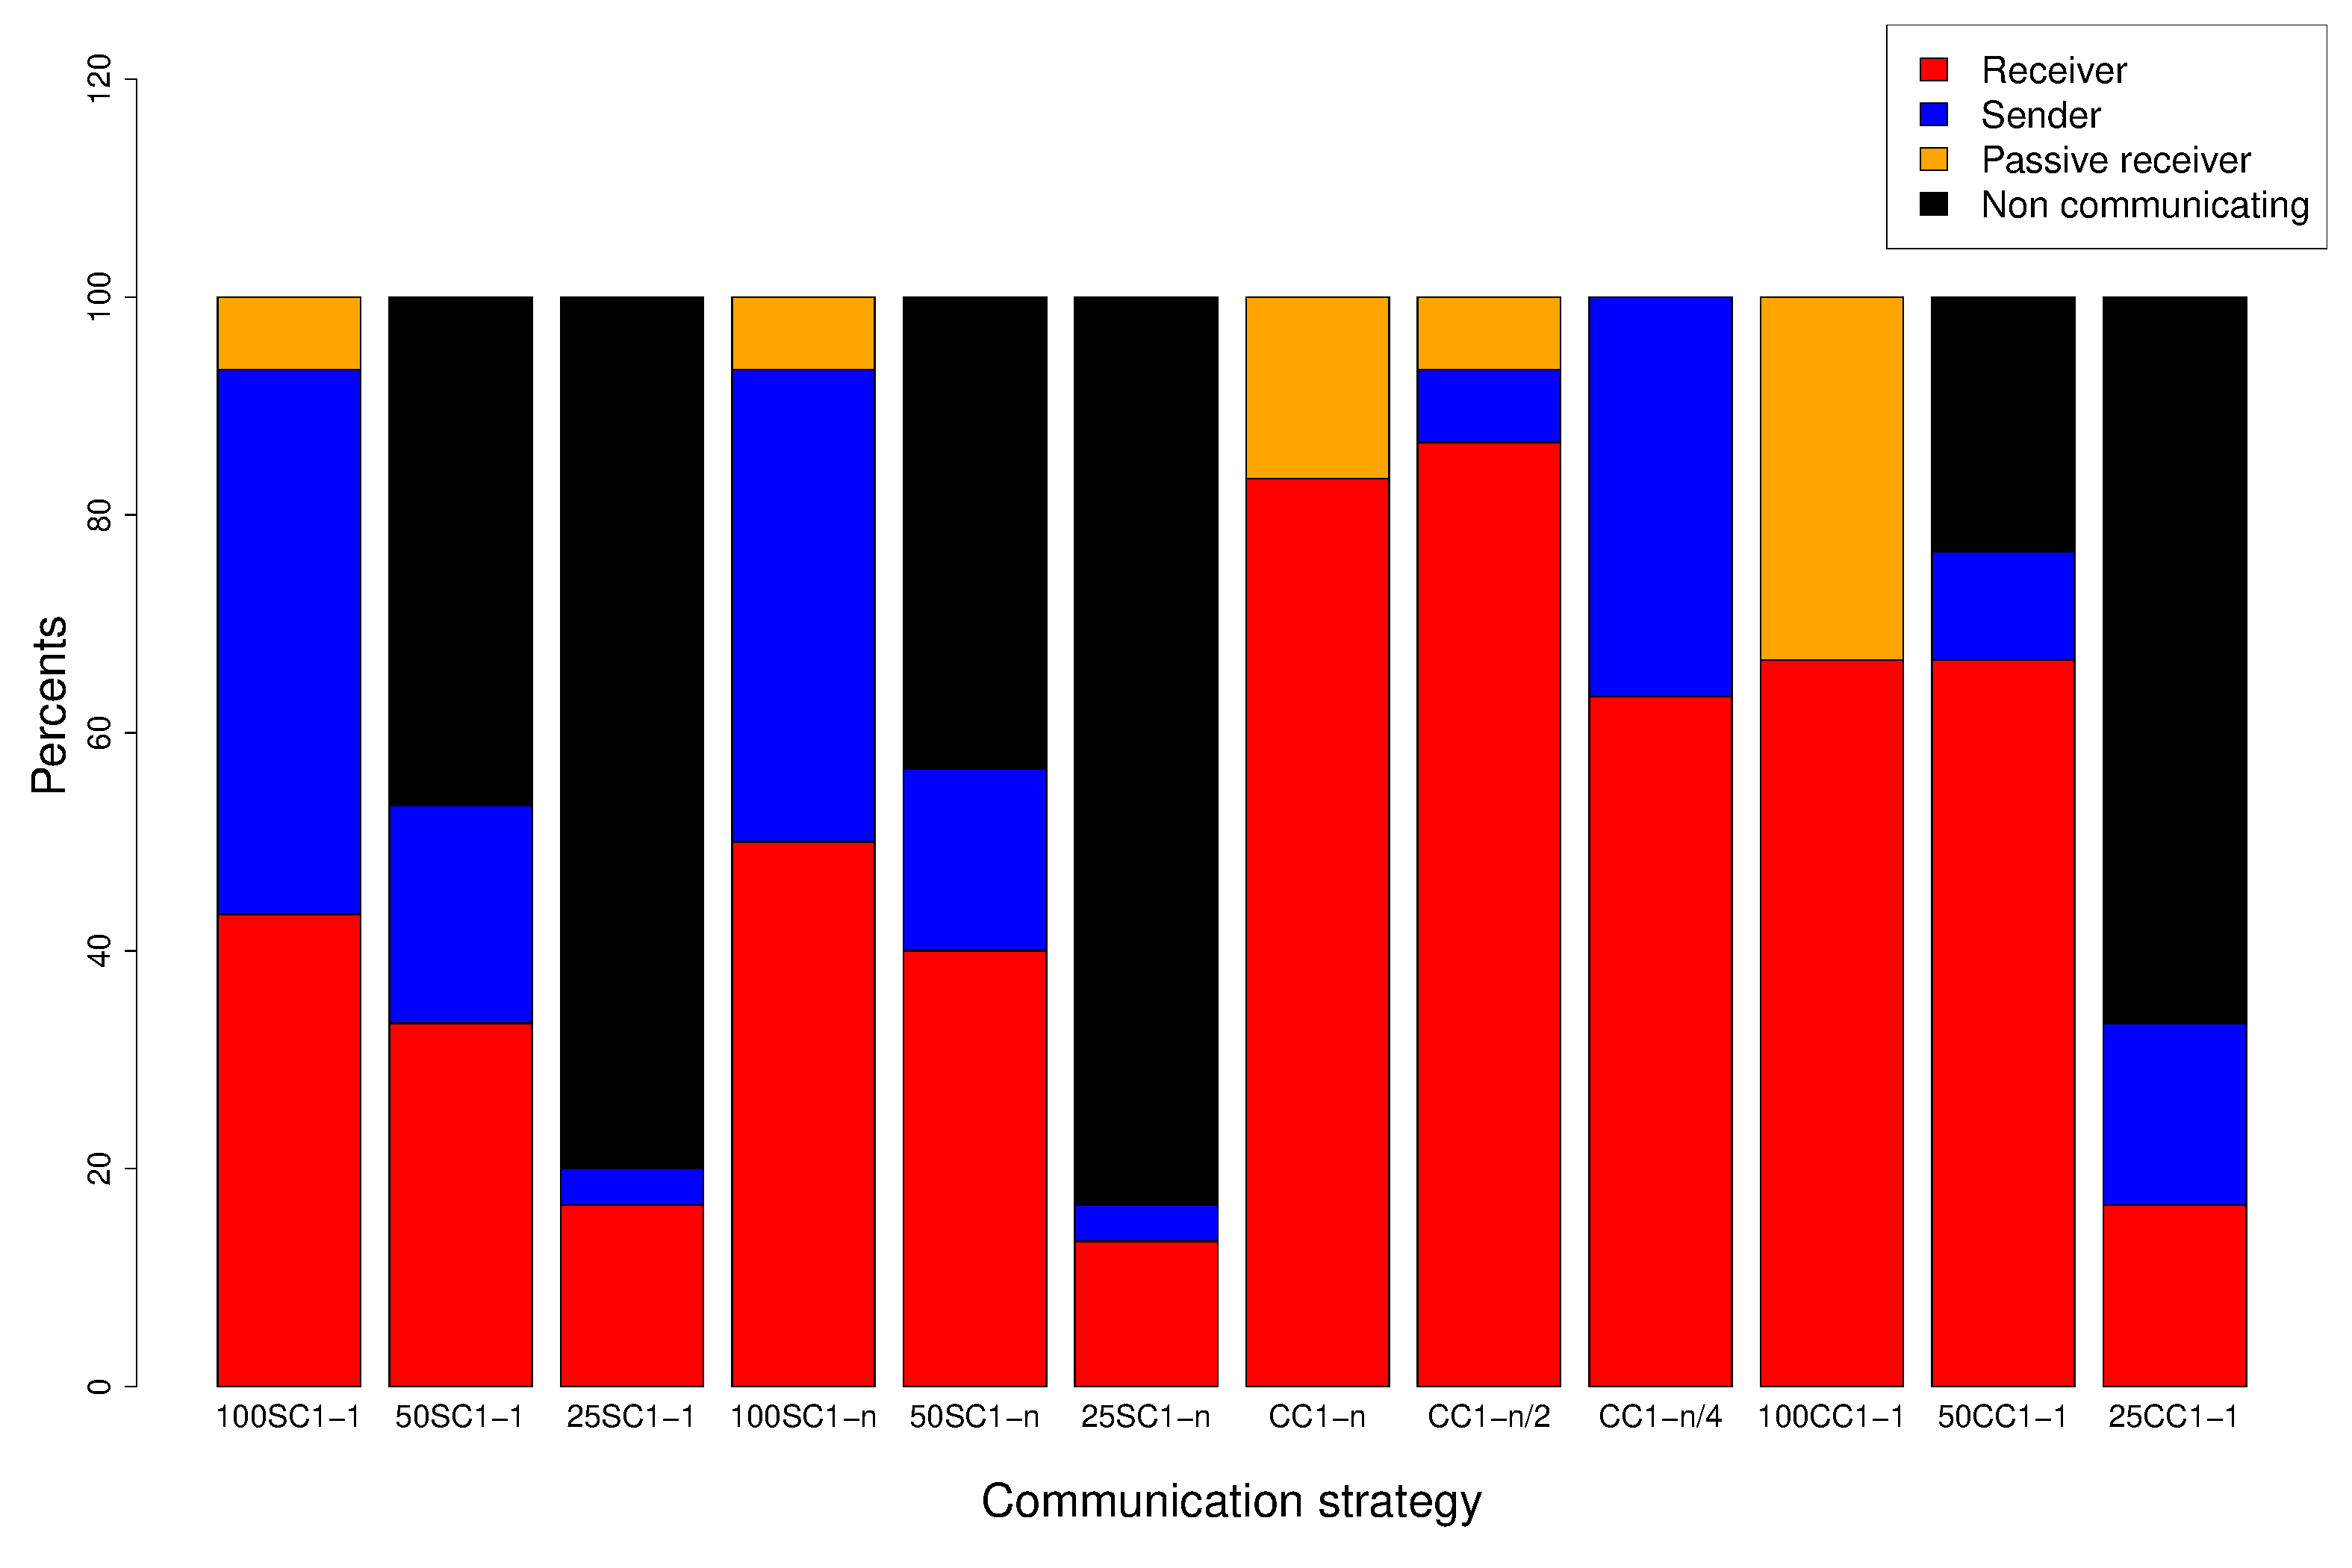
\includegraphics[width=0.8\textwidth]{g5_per_BP.pdf}
\caption{Solver proportion for each communication strategy to solve \SGP{} 5-3-7 using \posl}\label{barplot:5}
\end{figure}

\begin{figure}[!h]
\centering
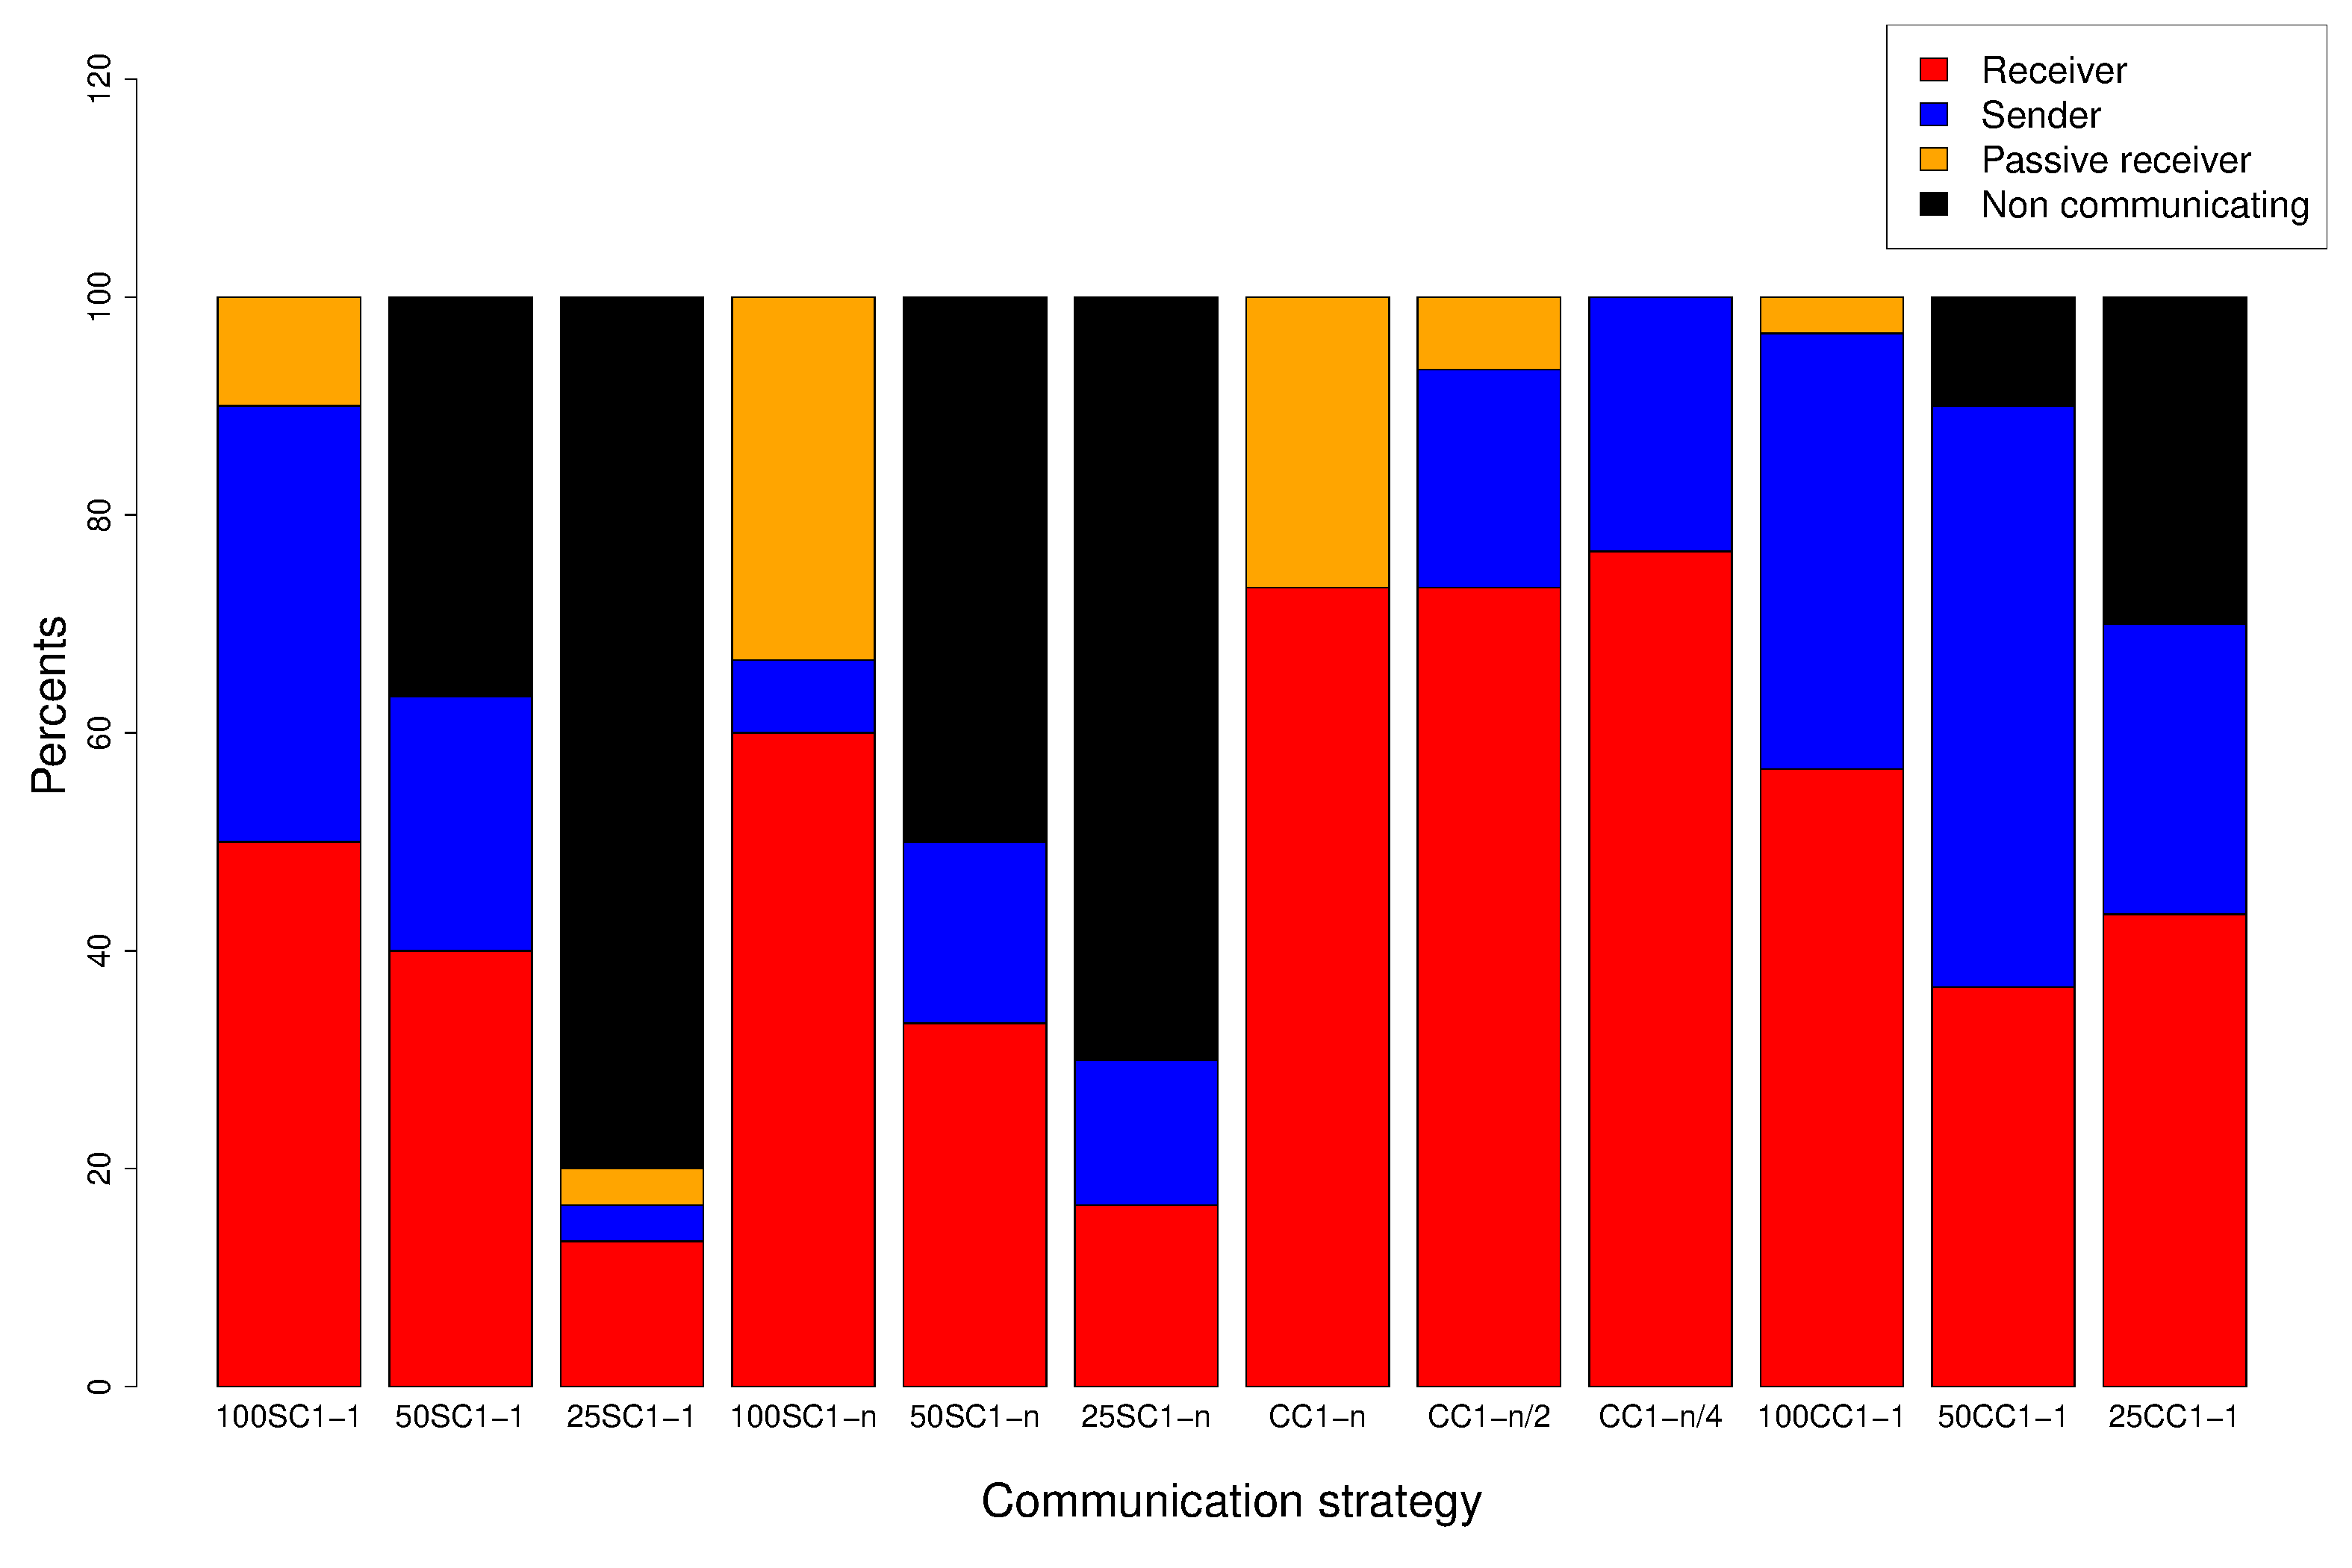
\includegraphics[width=0.8\textwidth]{g8_per_BP.pdf}
\caption{Solver proportion for each communication strategy to solve \SGP{} 8-4-7 using \posl}\label{barplot:8}
\end{figure}

\begin{figure}[!h]
\centering
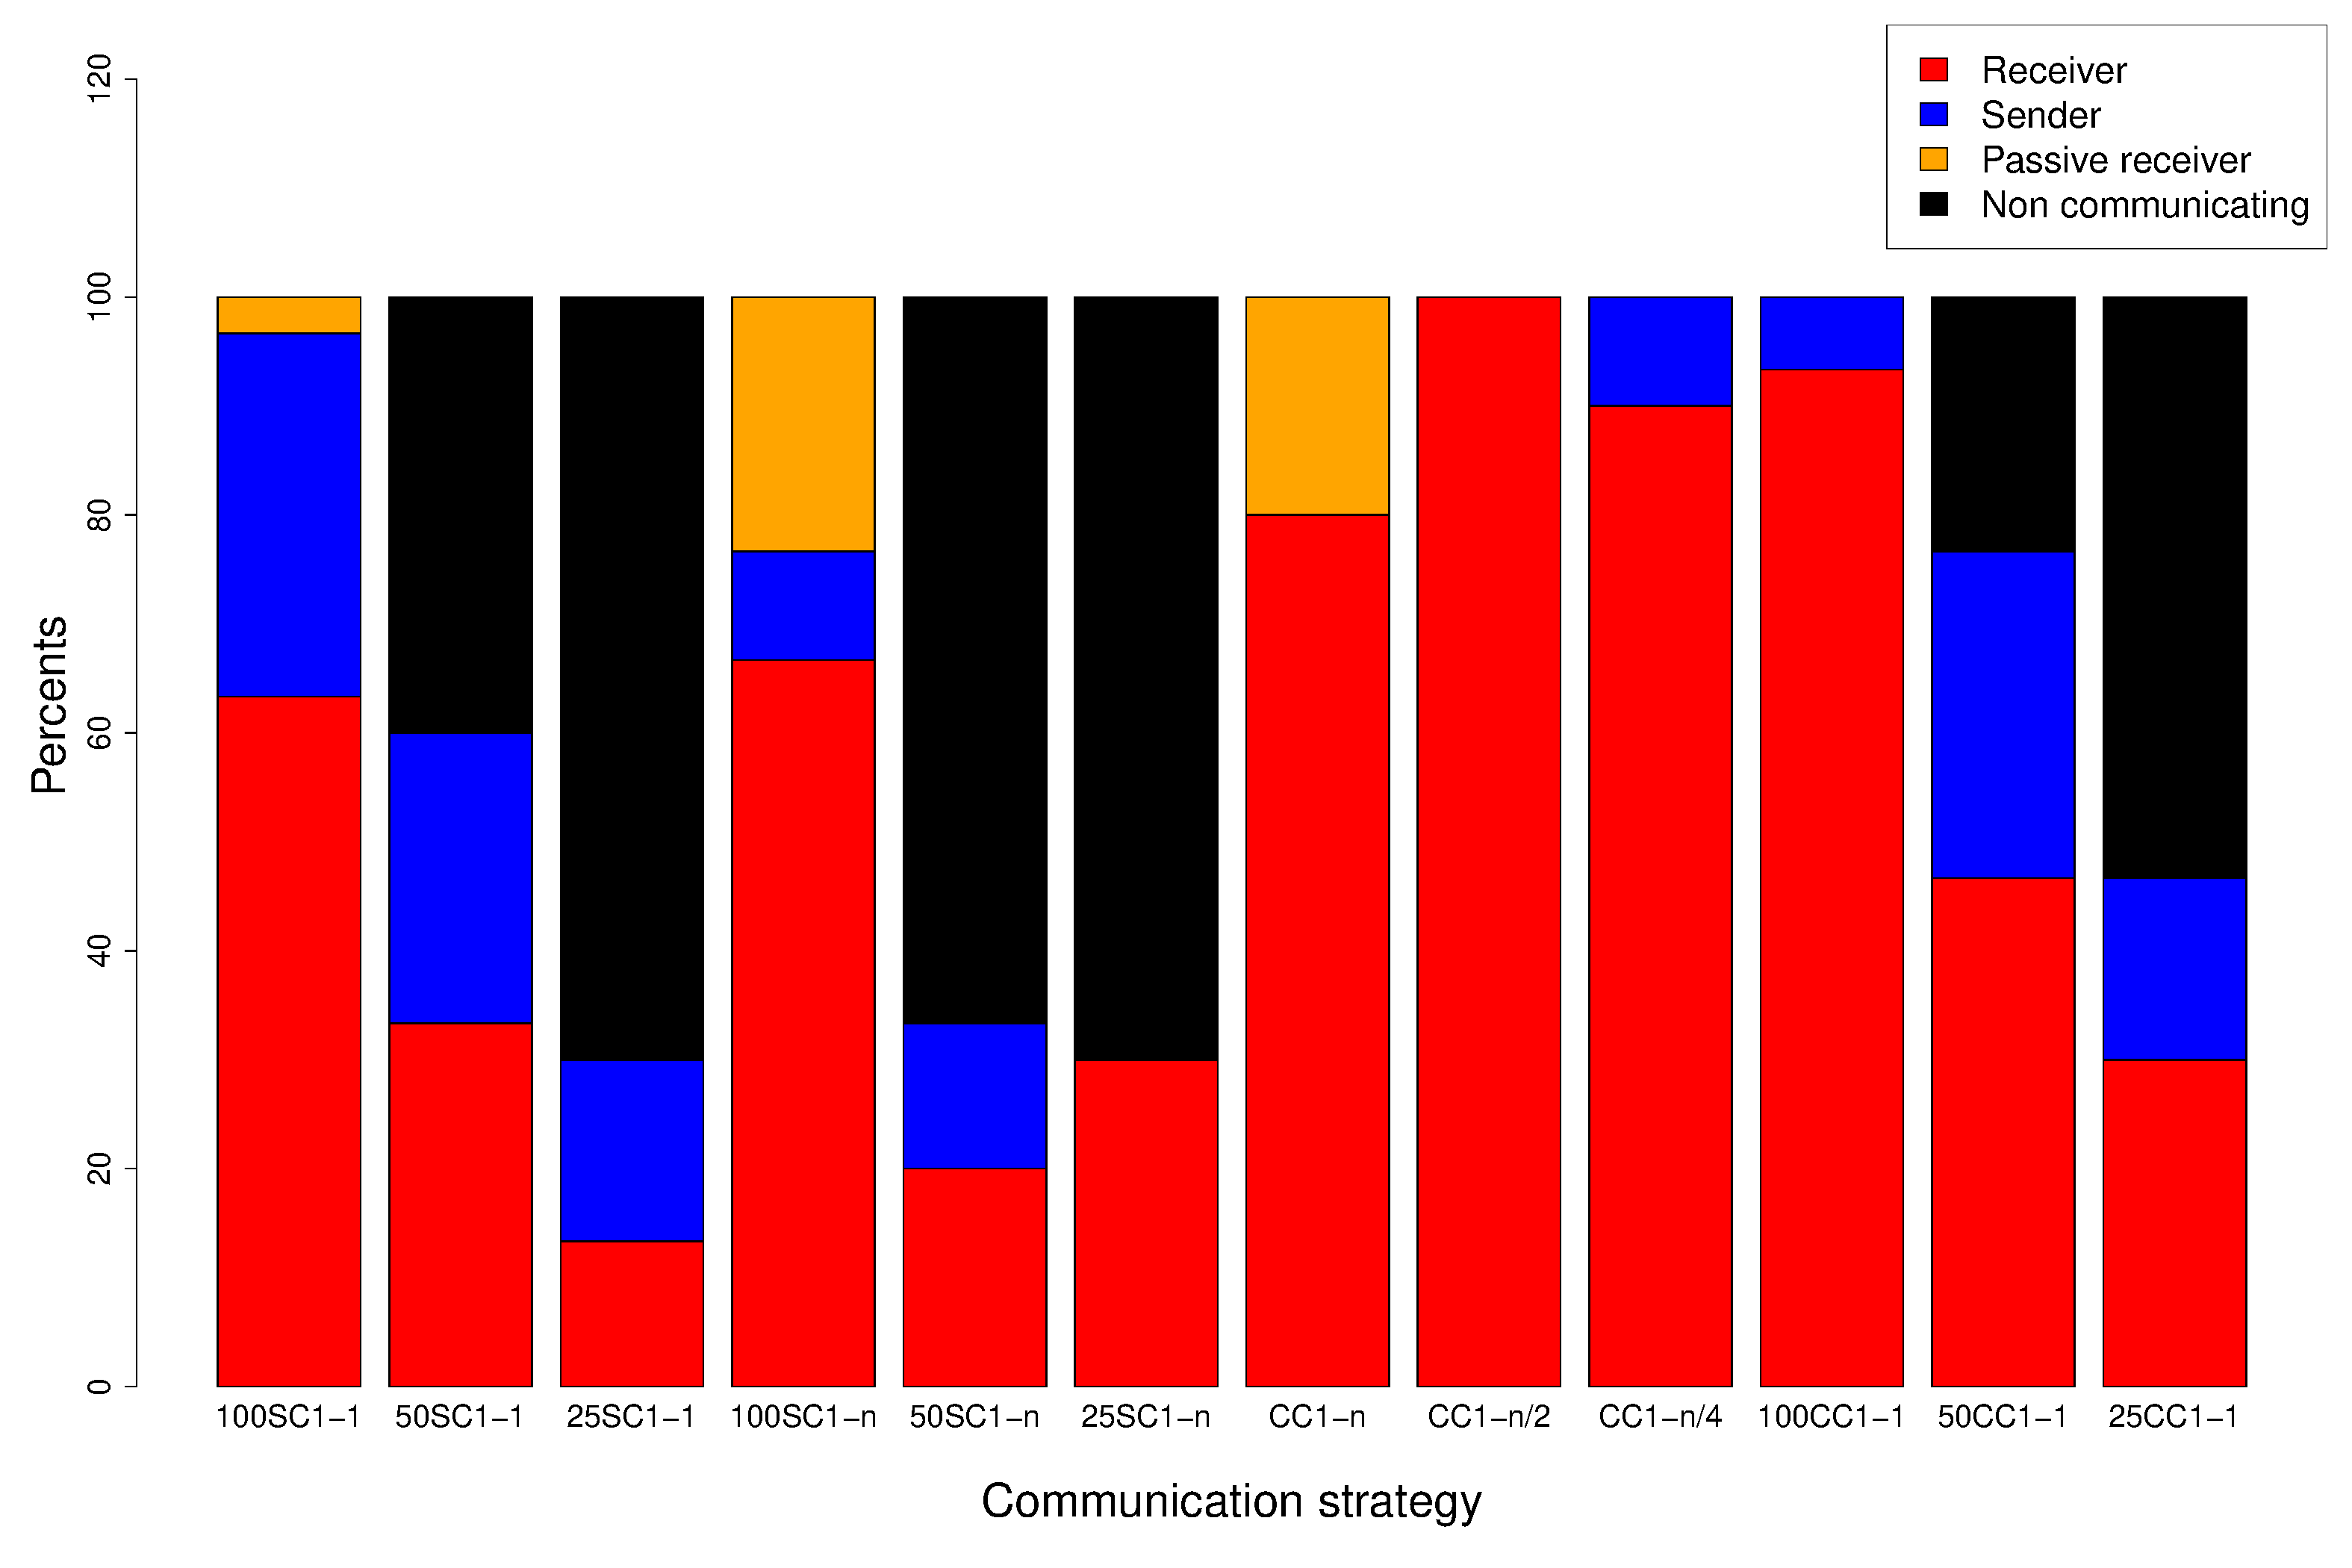
\includegraphics[width=0.8\textwidth]{g9_per_BP.pdf}
\caption{Solver proportion for each communication strategy to solve \SGP{} 9-4-8 using \posl}\label{barplot:9}
\end{figure}